\documentclass[12pt]{article}
\usepackage{graphicx}
\usepackage{tabularx}
\usepackage{multirow}
\usepackage[english]{babel}
\usepackage[absolute,overlay]{textpos}
\usepackage{verbatim}
\graphicspath{{image/}}
\usepackage{booktabs,subcaption,amsfonts,dcolumn}
\usepackage{cite}
\usepackage{blindtext}
\usepackage{titlesec}
\usepackage{array}
\usepackage[table]{xcolor}
\usepackage{colortbl}
\usepackage{diagbox}
\usepackage{hyperref}
\hypersetup{
	colorlinks,
	linkcolor={black!50!black},
	citecolor={blue!50!black},
	urlcolor={blue!80!black}
}
\usepackage{longtable}


\title{{\large \textbf{Palestine Ahliya Universty}
	\\
	\textbf{Faculty of Engineering and Information Technology}}\vspace{2cm}
	\\
	
	\textbf{{\Huge Patient Tracker}}\vspace{1cm}}
\author{\textbf{By}
	\\\\
	Hanna Odeh\qquad \qquad \quad
	Mohamed Hleesi\qquad \quad
	Roaa AbdEldayem
	\\\\
	\textbf{Supervisor}
	\\\\
	Ms.Rihabb Al-Salameen
}
\date{}

\begin{document}
	
	\begin{figure}[!t]
		\centering
		
\includegraphics[width=0.30\textwidth]{icon.png}
		\vspace{-1.5cm}
	\end{figure}

	\maketitle
	\thispagestyle{empty}
	
	\begin{center}
	\vspace*{1cm}A graduation project is submitted to the Department of Information Technology in partial fulfillment of the requirements for the degree of Bachelor of Science in Information Technology \vspace{0.2cm}
	\end{center}
	\begin{center}
		\date{\today}
		\newpage
	\end{center}
	\begin{center}
		\pagenumbering{roman}
		\textbf{DEDICATION}\\
		\begin{center}
		\end{center}
		First of all, we dedicate this graduation project to our parents, who endured all pains to make our dreams come true, and helped us to be here.
		
		To our supervisor Ms.Rihabb Al-Salameen who gave us all her efforts to complete this work.
		
		To our best friends everywhere. To our brothers and sisters.
		
		To all our teachers in our life.
		
		Love you all.
	\end{center}
	\newpage
	\begin{center}
		\textbf{ACKNOWLEDGMENT}\\
		\begin{center}
		\end{center}
		First of all, we are grateful to the Almighty God for making us the people we are today and giving us the strength and power to complete our mission.
		
		We would like to express our deepest appreciation to our parents, who prayed for us.
		
		Many thanks to our brothers and our sisters, who supported us all the time.
		we are also very grateful to our supervisor Ms.Rihabb Al-Salameen for her valuable supervision, guidance, and encouragement.
		
		We would also like to express our gratitude and appreciation to all our teachers in the IT department that helped us and showed us the guidance.
		
	\end{center}
	\newpage
	\begin{abstract}
		Many people suffer from diseases that can cause them additional and serious harm, for instance: Alzheimer patients with late stages may often forget their location, Hypoglycemic patients may have a sudden seizure where they immediately need suger and a piece of chocolate may save their lives, so our team is working on helping them by developing a Patient tracker (PT).\\
		
		 The proposed project is a mobile aplication for tracking location of patients. The purpose of the project is to improve patient care by providing real-time data on the location and health status of patients. The project will utilize GPS technology to track the location of the patient, and will also include features such as tracking vital signs (Blood presure, Oxygen saturation, Blood gloucose level, Heart rate, Insulin level) and medication adherence.
		The patient tracker app aims to help the healthcare providers and  tracks of patients. It will also provide patients with the ability to track their own health through the use of the mobile app. we will use the incremental agile methodology, which is well-suited for our system.\\
		
	\end{abstract}
	\newpage
	\tableofcontents
	\listoffigures
	\listoftables
	\newpage
	\pagenumbering{arabic}
	\section*{\begin{center}
			Chapter One
	\end{center}}
	\section{INTRODUCTION}
		\subsection{Introduction }
		    
			\quad In light of the remarkable progress of technology and the high rate of technology uses, many become dependent on technology, so much so that some of us can no longer manage or even get by without our phone, so we have decided to create a mobile app to help patients with some diseases that may cause additional harm, such as Alzheimer's and Diabetes.\\
			
			Patient tracker App technology is a rapidly evolving field that has the potential to transform the way that healthcare is delivered. These devices are designed to track the location and movements of patients in real time, using GPS (Google Maps), and may also have the capability to collect and transmit data about the patient's health, such as Blood presure, Oxygen saturation, Blood gloucose level, Heart rate and Insulin level. By downloading the patient tracker app on the healthcare's devices such as desktops, laptops, tablets or mobiles also, on patient's and family member mobiles and collecting the data of the vital signs from the apple watches, patients can access their health data and track their health and well-being in real-time, while also providing healthcare providers with valuable insights into their health status. In addition to tracking the location and health of patients, the patient tracker App can store and share medical records with patients, their families, and healthcare providers. This can help to ensure that all stakeholders have access to the most up-to-date and accurate information about the patient's health, and can facilitate more informed and collaborative decision-making about the patient's care.\\
			
			this project will benefit the medical and technology researchers sector, so after the project will be done and known this will help researchers to make extensive research about this. Trackers can provide real-time data on a patient's location and vital signs, which can help healthcare providers to respond more quickly to any changes in a patient's condition. also, Trackers can enable healthcare providers to communicate more effectively with patients, for example by sending reminders about appointments or medication and Alerting the family member and the patient to take medications relative to the medication schedule set by the doctor.\\
			

		\subsection{Literature Review}
			Tabel \ref{Literature Review} provides a summary of the different studies that have been conducted on patient trackers with location-tracking technology, including the purpose of the study, the features of the device, the benefits and limitations of using it, and the accuracy and reliability of the data collected. It also includes information on the privacy and security of the patient data, the costs and resources required for the device, and the level of acceptability and feasibility among patients and healthcare providers. By organizing this information in a comprehensive table, you can provide a clear and concise overview of the current state of research on patient trackers with location- tracking technology.
			\\\\\\\\\\
			
			 \newpage
			 \begin{table}[!h]
			 	\centering
			 	\caption{Literature Review}
			 	\label{Literature Review}
			 	\begin{tabular}{|p{2.6cm}|p{3.5cm}|p{3.5cm}|p{3.5cm}|} 
			 		\hline 
			 		\centering
			 		\cellcolor{lightgray}\backslashbox{diff}{Study}
			 		& 
			 			\centering\cellcolor{lightgray}\textbf{Evaluating the Effectiveness of a Mobile Health Tracking System for Chronic Disease Management}\cite{Study1}
			 		&
			 			\centering\cellcolor{lightgray} \textbf{The Impact of a Mobile Health Tracking App on Patient Outcomes}\cite{Study2}
		 			& 
		 				\cellcolor{lightgray}\textbf{A Systematic Review of Mobile Health Apps for Chronic Disease Management}\cite{Study3}\\
			 		\hline
			 		 \cellcolor{lightgray}\textbf{Purpose} & Clinical trial & Research project & Consumer product \\
			 		 \hline 
			 		 \cellcolor{lightgray}\textbf{Features} & Tracks location and vital signs & Tracks location and medication adherence & Tracks location and fitness data \\
			 		 \hline
			 		 \cellcolor{lightgray}\textbf{Benefits} & Improves patient care by providing real-time data & Reduces workload of healthcare providers by automating tracking and monitoring & Allows patients to track and improve their health on their own \\
			 		 \hline
			 		 \cellcolor{lightgray}\textbf{Limitations} & Potential for data errors & Potential for data errors & Limited clinical validation \\
			 		 \hline
			 		\cellcolor{lightgray}\textbf{Accuracy \quad/Reliability} & Validated by clinical trial & Data collected using validated methods & Data may not be as accurate as in clinical settings \\
			 		 \hline
			 		 \cellcolor{lightgray}\textbf{Privacy\qquad/Security} & Patient data encrypted and secure & Patient data encrypted and secure & Patient data may not be as secure as in clinical settings \\
			 		 \hline
			 		 \cellcolor{lightgray}\textbf{Costs\qquad/Resources} & Initial device cost and ongoing maintenance & Initial device cost and ongoing data management & Initial device cost and subscription fees \\
			 		 \hline
			 		\cellcolor{lightgray}\textbf{Acceptability \quad/Feasibility} &  High level of acceptance among patients and healthcare providers & High level of acceptance among patients, moderate acceptance among healthcare providers & Moderate level of acceptance among patients, low acceptance among healthcare providers \\
			 		 \hline
			 	\end{tabular}
			 \end{table}
		 	\newpage
		 	Patient Tracker App is specifically focused on the Bethlehem area, whereas the studies listed in the table have a wider geographical focus. This means that PT will be tailored to the specific needs and concerns of the Bethlehem community, which may differ from those of other communities. Additionally, PT will incorporate additional features and functionality that are not present in the studies listed in the table. For example, PT may include features such as real-time alerts for patients and caregivers, or integration with local healthcare resources and services. Overall, PT aims to provide a unique and comprehensive solution for the Bethlehem community that addresses the specific needs and concerns of patients, caregivers, and healthcare providers in the area.\\
		\subsection{Project Scope}
			\quad The scope of the patient tracker project in Bethlehem is to improve the management of patients with chronic conditions, enhance the efficiency of healthcare delivery, and improve communication and collaboration between patients, doctors, and other healthcare providers. The project aims to provide real-time tracking of patients’ locations and health status, as well as store and share medical records and other important information. This will benefit both doctors and patients by enabling more timely and effective care, as well as providing patients with greater control and autonomy over their health. In addition, the project will benefit the medical sector by providing valuable insights and data that can inform research and improve the quality of care for all patients.\\
			
			
			\textbf{\underline{The included functions of this system: }}\\
			\begin{itemize}
				\item This system depends on or works on hosting services for the medical sector, patients, and their families that suffer, such as tracking and locating the patient's current place, viewing the patient’s illness record, checking his bumps and oxygen, sending notifications and alarming,  etc. 
				\item As it will allow patients with their families to access the app, So first they must register to create a personal account that will be informed by the medical ministry to insure that they are allowed to use this app and the sensitive information or not, it will be registering an ID number, first name, last name, date of birth, gender, place of birth, email, password, personal phone number, their location or their place of residence, two of patient’s relative name and contact information to keep them in touch, that information are all required to fill in their registration form, this system will allow changing or updating some information such as phone number and place of residence. 
				\item After all, they will officially have a personal account on our application, where the citizen will log in with the ID number and password, and then allow the user to visit the registry, and check the sites and biometrics. 
				This application will be available 24 hours, all the time, in case the patient lost network connection then his last location will be saved and an alert will be sent to the family member  with the last location where he was.
			\end{itemize}
		
			\begin{center}
			\end{center}
			\textbf{\underline{The excluded functions:}} \\
			\begin{itemize}
				\item Medication Reminders: Set reminders for timely medication.
				\item Appointment Management: Schedule and manage medical appointments.
				\item Data Visualization: Visualize health data.
				\item Health Education: Provide educational resources.
				\item Personalized Recommendations: Receive personalized health recommendations.
				
			\end{itemize}
			 
			\textbf{\underline{Clients:}}\\
			
			This project targets specific patients throughout Bethlehem, and a number of experts, clinics, hospitals, and investors are working on it to help and support all the patients and their families to use and achieve the main goal of protecting and caring for these patients. 

		\subsection{Problem Statement}
			
			\quad There is a lack of effective methods for healthcare providers to monitor and track the location and health status of patients in real-time. This can lead to poor health outcomes and high healthcare costs, as well as difficulties in providing timely care in emergencies, for instance diabetes patients may have a sudden seizure where they immediately need sugar and a piece of chocolate may save their lives and Alzheimer patients with late stages may often forget their location.\\
			
			PT aims to create a mobile application that helps patients and their families physically, psychologically, and socially, as it will reduce the number of injuries, danger, and deaths that patients may be exposed to, and it will reduce psychological anxiety and phobia the social status of patients and their families, by tracking the location and vitals of patients, displaying their health conditions, what they may be exposed to, and their medical records that will be stored in the application. Finally, it is important to address the privacy and security concerns surrounding the use of patient tracker technology by implementing appropriate safeguards and measures to protect the privacy and security of patient data. This may include obtaining consent from patients before collecting or sharing their data, implementing measures to encrypt and secure patient data, and ensuring that patient data is only accessed by authorized personnel. By addressing these concerns, it is possible to build trust and confidence in the use of patient tracker technology and to encourage more widespread adoption of these devices.
			
		\subsection{Project Objectives}
		The specific objectives of the PT system are as follows:
		\begin{enumerate}
			\item To improve adherence to treatment plans by providing real-time monitoring and reminders for patients.
			\item To improve the efficiency and effectiveness of healthcare providers by providing real-time data on patient health and location.
			\item To improve the safety and security of patients, especially those with cognitive impairments, by providing location tracking and emergency alerts.
			\item To improve the timeliness of care in emergency situations by providing real-time location tracking of patients.
			\item To reduce healthcare costs by improving health outcomes and reducing the need for hospital visits or other costly interventions.
		
		\end{enumerate}
		\subsection{Project Benefits}
			There are several potential benefits of using patient tracker technology and connecting it with a patient's medical record in the healthcare setting:
			
			\begin{enumerate}
				\item Improved patient outcomes: By providing real-time monitoring of patient health data, patient tracker technology can help to identify early warning signs of deterioration and allow for timely intervention. This can help to prevent complications and hospitalizations and may result in improved patient outcomes.
				\item Enhanced patient engagement: By providing patients with access to their own health data and allowing them to track their own health and well-being, patient tracker with location tracker technology can help to increase patient engagement in their own care. This can lead to better self-management of chronic conditions and may result in improved health behaviors.
				\item Increased efficiency and cost-effectiveness: By providing real-time data on patient health, patient tracker with location tracker technology can help to reduce the need for unnecessary hospitalizations and emergency department visits, which can result in cost savings for the healthcare system.
				\item Improved communication and collaboration: By connecting patient tracker with location tracker technology with a patient's medical record, healthcare providers can have access to more comprehensive and up-to-date information about the patient's health, which can facilitate more informed and collaborative decision-making about the patient's care.
				\item Enhanced patient privacy and security: By implementing appropriate safeguards and measures to protect the privacy and security of patient data, patient tracker with location tracker technology can help to build trust and confidence in the use of these devices among patients and their families.
			\end{enumerate}
		
			Overall, the use of patient tracker with location tracker technology and the connection of these devices with a patient's medical record has the potential to transform the way that healthcare is delivered and to improve the quality, efficiency, and cost-effectiveness of healthcare for patients and their families.
		\subsection{Project Methodology}
	
			\quad Many software methodologies have emerged for the development of software systems, such as waterfall, agile, ... etc. For the development of our system, we will follow the agile methodology using the incremental development strategy. The following justifies the selection of agile in particular:
				\begin{enumerate}
				\item Incremental agile is a flexible and adaptable approach to project management that allows for ongoing iteration and improvement. This is particularly useful for the patient tracker project that involves researching and reviewing a complex and rapidly evolving area such as patient tracker technology.
				\item Incremental agile allows for a flexible and iterative approach to the patient tracker project, with a focus on delivering small increments of value at regular intervals. This can help to ensure that the project remains on track and that the deliverables are completed promptly.
				\item Incremental agile emphasizes collaboration and communication between team members, which is important for the patient tracker project that involves multiple stakeholders such as patients, healthcare providers, and researchers.
				\item Incremental agile allows for a high degree of transparency and visibility into the patient tracker project, with regular check-ins and progress updates that help to keep all stakeholders informed about the status of the project.
				\item Incremental agile is well-suited to the patient tracker project that involves a high level of uncertainty or complexity, as it allows for ongoing adjustment and adaptation to changing circumstances and requirements.
				\item Agile helps in remaining within the boundaries of budget assigned for PT, as each feature of system are shown to the customer after it is developed and before moving forward to other major functionality. This will prevent the development of unneeded features.
				\end{enumerate}
				
			Overall, we believe that incremental agile is the best project methodology for the patient tracker, as it allows for flexibility, collaboration, and transparency, and is well-suited to the complex and rapidly evolving nature of this technology.
						
		\subsection{Proposed Working Plan}
		
		\quad Collective work is done on the project as face-to-face meetings and meetings are held on the google to present the project and meet the customers who will use the system and follow up with them in every step to obtain the functional requirements of the system.
			
		\subsection{Project Constraints }
		
			\quad Project constraints are factors that can limit or restrict the scope, resources, ortimeframe of a project. Some potential constraints for a patient tracker projectmight include:
			\begin{enumerate}
				\item Time: The project may be constrained by a limited time frame, which could impact the scope of the project and the amount of research that can be conducted, PT must be implemented and deployed within a year, which is the year specified by the deadline assigned to graduation.
				\item Budget: The project may be constrained by a limited budget, we have to work on developing the system with this limited and confined budget.
				\item Data availability: One of the limitations that may face the development of the system is the availability of medical data for use in the system.
				\item Access to participants: There may be challenges in recruiting and accessingpatients or healthcare providers who are willing and able to participate in theproject. This could impact the ability to gather data or to get feedback onthe use of patient trackers with location tracker technology.
				\item Ethical considerations: There may be ethical considerations surrounding theuse of patient trackers with location tracker technology, such as privacy andsecurity concerns, that need to be taken into account when conducting theresearch and preparing the presentation. For example, it may be necessaryto obtain consent from patients and healthcare providers before collecting orsharing their data or to implement measures to protect the privacy andsecurity of patient data.
				\item Security: Patient data collected by the tracker system is often sensitive and personal in nature, that patient data could be accessed or stolen by unauthorized individuals, either through hacking or other types of data breaches. The data can be exposed to cyber threats such as malware or phishing attacks to ensure the security and integrity of the data being collected and transmitted.
			\end{enumerate}
		\subsection{Summary}
		
		\quad This project aims to provide a comprehensive overview of the current state of research on patient tracker technology and its potential applications in the healthcare setting. Overall, the use of the patient tracker project and the connection of these devices with a patient's medical record has the potential to transform the way that healthcare is delivered and to improve the quality, efficiency, and cost-effectiveness of healthcare for patients and their families.
		\newpage
	\section*{\begin{center}
			Chapter Two
	\end{center}}
	\section{SYSTEM ANALYSIS }
		\subsection{Introduction}
			\quad System analysis is a crucial step in the development of any project, including a patient tracker and location tracking project. It involves examining the current system, identifying its weaknesses and strengths, and determining how it can be improved, system analysis involves a detailed study of the project requirements, including the functional and non-functional requirements, as well as the business and technical constraints.
			
		\subsection{Project Implementation Options}
			\textbf{There are several benefits to choosing mobile as the platform for your project implementation:}
			\begin{enumerate}
				\item Wide reach: Mobile devices are widely used and can reach a large audience. This makes it easier for you to reach your target users and customers \cite{usingsmartphone}.
				\item Convenience: Mobile devices are portable and can be accessed anytime, anywhere. This makes it easier for users to access your project on the go and at their own convenience\cite{schadler2012mobile}.
				\item Cost-effective: Developing a mobile app can be more cost-effective compared to other platforms, especially if you want to reach a large audience.
				\item Personalization: Mobile apps can be designed to provide a personalized experience to users, which can increase user engagement and loyalty.
				\item Integration with other features: Mobile apps can be integrated with various features such as push notifications, GPS, and cameras, which can enhance the functionality of your project.
				\item Access to hardware: Mobile devices come with a range of hardware such as sensors and cameras, which can be leveraged to enhance the user experience and functionality of your project.
				\item Offline functionality: Mobile apps can be designed to work offline, which can be useful in situations where internet connectivity is limited.
				\item Fast development: Mobile apps can be developed and deployed faster compared to other platforms, which can help you bring your project to market quickly.
			\end{enumerate}
			\textbf{There could be various reasons why a website was not chosen as the platform for your project implementation. Some possible reasons could include:}
			\begin{enumerate}
				\item Limited reach: Websites are accessed through a web browser and require an internet connection. This means that they may not be accessible to users in areas with limited or no internet connectivity.
				\item Limited functionality: Websites are generally limited in terms of the features and functionality they can offer compared to mobile apps. For example, a website may not be able to access device hardware such as the camera or GPS.
				\item Poor user experience: Websites may not provide the same level of user experience as mobile apps, which can lead to lower user engagement and satisfaction.
				\item Slow development: Developing a website can take longer compared to mobile app development, especially if you want to include advanced features and functionality.
				\item High costs: Developing a website can be more expensive compared to mobile app development, especially if you want to include advanced features and functionality.
				\item Limited personalization: Websites may not be able to provide the same level of personalization as mobile apps, which can lead to a less engaging user experience.
				\item Lack of integration with other features: Websites may not be able to integrate with other features such as push notifications, which can limit their functionality.
				\item Lack of offline functionality: Websites generally require an internet connection to function, which can be a limitation in situations where internet connectivity is limited.
			\end{enumerate}
		\textbf{There could be various reasons why a desktop app was not chosen as the platform for your project implementation. Some possible reasons could include:}
			\begin{enumerate}
				\item Limited reach: Desktop apps are only accessible on desktop or laptop computers, which means that they may not be accessible to users on mobile devices or tablets.
				\item Limited functionality: Desktop apps are generally limited in terms of the features and functionality they can offer compared to mobile apps. For example, a desktop app may not be able to access device hardware such as the camera or GPS.
				\item Poor user experience: Desktop apps may not provide the same level of user experience as mobile apps, which can lead to lower user engagement and satisfaction.
				\item Slow development: Developing a desktop app can take longer compared to mobile app development, especially if you want to include advanced features and functionality.
				\item High costs: Developing a desktop app can be more expensive compared to mobile app development, especially if you want to include advanced features and functionality.
				\item Limited personalization: Desktop apps may not be able to provide the same level of personalization as mobile apps, which can lead to a less engaging user experience.
				\item Lack of integration with other features: Desktop apps may not be able to integrate with other features such as push notifications, which can limit their functionality.
				\item Lack of offline functionality: Desktop apps generally require an internet connection to function, which can be a limitation in situations where internet connectivity is limited.
			\end{enumerate}
		
		There are several mobile application frameworks available, each with its own strengths and differences. Here is a brief description of some popular mobile application frameworks:
		\begin{table}[!h]
			\centering
			\caption{Difference Between Mobile Application FrameWorks\cite{nawrocki2021comparison}}
			\begin{tabular}{|p{3cm}|p{2cm}|p{2cm}|p{2cm}|p{2cm}|}
				\hline
				\rowcolor{lightgray}
				\backslashbox{diff}{Frame} & \textbf{Native\quad IOS} &\textbf{Native\quad Android} & \textbf{React\quad Native} & \textbf{Flutter} \\
				\hline
				\cellcolor{lightgray}\textbf{Operation}\qquad System & Apple Only & Android Only & IOS, Android, Web & IOS, Android, Web\\
				\hline
				\cellcolor{lightgray}\textbf{Language} & Swift & Kotlin & Java Script &Dart\\
				\hline
				\cellcolor{lightgray}\textbf{Performance} & Very High & Very High & High & High\\
				\hline
				\cellcolor{lightgray}\textbf{Cost And Time} & More Expensive and Slower & More Expensive and Slower & Cheaper And Faster & Cheaper And Fast\\
				\hline
				\cellcolor{lightgray}\textbf{Popular Apps} & Safari, iTunes, Messages & SwiftKey, Pocket Casts & Facebook, Instagram, Airbnb & Alibaba, Tencent, Google Ads\\
				\hline
				\cellcolor{lightgray}\textbf{Community Support} & Very Popular & Very popular & Very Popular & Popular\\
				\hline
			\end{tabular}
		\end{table}
		\subsection{The Proposed System}
			\textbf{A proposed system for a patient tracker includes the following features:}
			\begin{enumerate}
				\item Patients can register and create an account on the platform, which will allow them to access their medical records and track their health status.
				\item Patients can view and update their medical records, including information about their medical history, allergies, medications, and test results.
				\item Patients can schedule appointments with their healthcare provider and receive reminders about upcoming appointments.
				\item Patients can track and report their symptoms, which can help their healthcare provider identify any potential health issues.
				\item Patients can track and manage their medications, including the dosage and frequency of their medications.
				\item Patients can track their health metrics such as blood pressure, weight, and glucose levels, and view their progress over time.
				\item Patients can access educational resources and tips on managing their health and preventing potential health issues.
				\item Patients can communicate with their healthcare provider through a secure messaging system, which can help them get answers to their questions and concerns.
				\item Location tracking, patients can opt-in to location tracking, which will allow their healthcare provider to track their location and ensure they are receiving the appropriate care.
				\item Integration with wearable devices: The platform can be integrated with wearable devices such as fitness trackers, which can provide additional health data for patients and their healthcare providers.
				\item The emergency alert system, patients can set up an emergency alert system that will alert their healthcare provider if they are in a potentially dangerous situation or if they need immediate medical attention.
			\end{enumerate}
		\begin{center}
			\newpage
		\end{center}
		\subsection{System Requirements}
			\subsubsection{Functional requirements}
				\begin{itemize}
					\item Patient registration: Patients should be able to create an account on the platform and provide their personal and medical information.
					\item Medical record management: Patients should be able to view and update their medical records, including information about their medical history, allergies, medications, and test results.
					\item Appointment scheduling: Patients should be able to schedule appointments with their healthcare provider and receive reminders about upcoming appointments.
					\item Symptoms tracker: Patients should be able to track and report their symptoms, which can help their healthcare provider identify any potential health issues.
					\item Medication management: Patients should be able to track and manage their medications, including the dosage and frequency of their medications.
					\item Health tracking: Patients should be able to track their health metrics such as blood pressure, weight, and glucose levels, and view their progress over time.
					\item Health tips and resources: Patients should be able to access educational resources and tips on how to manage their health and prevent potential health issues.
					\item Secure messaging: Patients should be able to communicate with their healthcare provider through a secure messaging system, which can help them get answers to their questions and concerns.
					\item Location tracking: Patients should be able to opt-in to location tracking, which will allow their healthcare provider to track their location and ensure they are receiving the appropriate care.
				\end{itemize}
			\subsubsection{Non-functional requirements}
				\begin{itemize}
					\item Security: The platform should be secure and protect patient data from unauthorized access, 
					Security is important for any project, but especially for a patient tracker with a location tracker project, because it involves the collection, storage, and dissemination of sensitive personal and health information. Ensuring the security of this information is essential to protect the privacy and confidentiality of the patient and to ensure that the data is accurate and reliable.
					\item Scalability: The platform should be able to handle a large number of users and handle increased traffic as needed.
					\item Performance: The platform should have fast load times and be able to handle multiple requests simultaneously.
					\item Usability: The platform should be easy to use and navigate for patients of all ages and tech-savviness.
					\item Compatibility: The platform should be compatible with a range of devices, including smartphones, tablets, and desktop computers.
					\item Maintenance: The platform should be regularly maintained and updated to ensure it is functioning properly.
				\end{itemize}
		
		\subsection{Feasibility Study}
			\subsubsection{Economic Feasibility}
			
				\quad Economic feasibility is one of the most important factors that drive the implementation of the project or not to implement it, and in order for the work team to spread the product effectively and at the lowest costs, it is necessary to conduct a study of all economic costs related to project development and implementation.
				
				\begin{table}[!h]
					\centering
					\caption{Economic Feasibility Study}
					\begin{subtable}{\textwidth}
						\centering
						\caption{Software}
						\begin{tabular}{|p{3.4cm}|p{2.1cm}|p{2cm}|p{1.5cm}|p{1.5cm}|}
							
							\hline
							\rowcolor{lightgray}
						 	\textbf{service Name} & \textbf{Number of services} & \textbf{Cost per one} & \textbf{Total cost} & \textbf{links}\\
						 	\hline
						 	Windows 11 pro & 3 & 29.99\$ & 89.97\$ & \href{https://instantlegit.com/product/microsoft-windows-11-professional-win-11-pro-license-code-key-original-new/}{microsoft}\\
						 	\hline
						 	VS Code & 3 & Free & Free & \href{https://code.visualstudio.com/}{VSCode} \\
						 	\hline
						 	Dart SDK & 3 & Free & Free & \href{https://dart.dev/get-dart}{Dart}\\
						 	\hline
						 	Flutter SDK & 3 & Free & Free & \href{https://docs.flutter.dev/get-started/install}{Flutter}\\
						 	\hline
						 	Android Studio & 3 & Free & Free & \href{https://developer.android.com/studio?gclid=CjwKCAiA2L-dBhACEiwAu8Q9YPOXet45HbMjGcjlZae74qH_Gq85oXOyydm8-tyNoXUi6DiOTKbEmRoC7FYQAvD_BwE&gclsrc=aw.ds}{Android Studio}\\
						 	\hline
						 	Compiler MIKTex , Editor TeXstudio & 3 & Free & Free &\href{http://www.miktex.com/}{MikTex}, \href{https://www.texstudio.org/}{Texstudio}\\
						 	\hline
						 	MS Office  2019 & 3 & 18.34\$ & 55.02\$ & \href{https://www.microsoft.com/en-us/}{microsoft} \\
						 	\hline
						 	EdrawMax & 3 & 69\$ & 207\$ & \href{https://www.edrawsoft.com/pricing-edrawmax.html}{edrawsoft}\\
						 	\hline
						\end{tabular}
					\end{subtable}
					\begin{center}
					\end{center}
					\begin{subtable}{\textwidth}
					\centering
					\caption{Hardware}
					\begin{tabular}{|p{3cm}|p{2.1cm}|p{1.9cm}|p{1cm}|c|}
						\hline
						\rowcolor{lightgray}
						\textbf{Device Name} & \textbf{Number of devices} & \textbf{Cost per one} & \textbf{Total cost} & \textbf{Links}\\
						
						\hline
						laptop (Medium specification) & 3 & 759\$ & 2277\$ & \href{https://www.amazon.com/Acer-Notebook-i7-1165G7-Keyboard-Fingerprint/dp/B0BP9LWT76/ref=sr_1_1_sspa?keywords=laptop%2Bcore%2Bi7&qid=1672501208&sprefix=laptop%2Bcore%2Caps%2C249&sr=8-1-spons&smid=A3QR4864ATM9Z9&spLa=ZW5jcnlwdGVkUXVhbGlmaWVyPUExTENBUEQyNVI2U0NQJmVuY3J5cHRlZElkPUEwNjI1Mjk1M1Q0TFdXMUFFUkpEJmVuY3J5cHRlZEFkSWQ9QTA4NzkxODkxNzBCWTBKT0NTUEpZJndpZGdldE5hbWU9c3BfYXRmJmFjdGlvbj1jbGlja1JlZGlyZWN0JmRvTm90TG9nQ2xpY2s9dHJ1ZQ&th=1}{laptop}\\
						\hline
						Smart-phone (Medium specification)  & 3 & 281\$  & 843\$ & \href{https://www.amazon.com/Xiaomi-Redmi-Note-11-Pro/dp/B09TKFFS23/ref=sr_1_3?keywords=note%2B11%2Bpro&qid=1672501497&sprefix=note%2B11%2B%2Caps%2C254&sr=8-3&th=1}{SmartPhone}\\
						\hline
						Smart-watch (High specification) & 3 & 223\$ & 669\$ & \href{https://www.amazon.com/Apple-Watch-Smart-Midnight-Aluminum/dp/B0BDJ1MVBV/ref=sr_1_1?keywords=apple%2Bwatch&qid=1672501658&sprefix=apple%2Caps%2C246&sr=8-1&th=1}{Smartwatch}\\
						\hline
					\end{tabular}
				\end{subtable}
				\end{table}
			\newpage
				\begin{center}
				\newpage
				\end{center}
			
				\subsubsection{Technical Feasibility Study}
				\begin{table}[!h]
					\centering
					\caption{Technical Feasibility Study}
					\begin{tabular}{|l|l|}
						\hline
						\rowcolor{lightgray}
						\# & \textbf{Necessary Abilities and Skills}\\
						\hline
						\cellcolor{lightgray}\textbf{1.} &  Programming Language \\
						\hline
						\cellcolor{lightgray}\textbf{2.} & Back-End Development \\
						\hline
						\cellcolor{lightgray}\textbf{3.} & User Interface Design ( UI )\\
						\hline
						\cellcolor{lightgray}\textbf{4.} & Software Engineering \\
						\hline
						\cellcolor{lightgray}\textbf{5.} & Problem Solving\\
						\hline
					\end{tabular}
				\end{table}
			\subsubsection{Human Resources Feasibility Study }
		\begin{table}[!h]
			\centering
			\caption{Human Resources}
			\begin{tabular}{|c|p{3.4cm}|l|l|}
				\hline
				\rowcolor{lightgray}
				\# & \textbf{Occupation} & \textbf{The number of people} & \textbf{Salary} \\
				\hline
				\cellcolor{lightgray}\textbf{1} & Software engineer and interface designer & 1 & 1300\$\\
				\hline
				\cellcolor{lightgray}\textbf{2} & Mobile application developer & 1 & 1000\$ \\
				\hline
				\cellcolor{lightgray}\textbf{3} &  Backend developer & 1 & 1000\$ \\
				\hline
			\end{tabular}
		\end{table}
			
		\begin{center}
			\newpage
		\end{center}
		\subsubsection{Scheduling Feasibility Study}
			\begin{table}[!h]
				\centering 
				\caption{Scheduling Feasibility Study}
				\begin{subtable}{\textwidth}
					\centering
					\caption{Project Plan for First Semester.}
					\begin{tabular}{|c|l|c|}
						
						\hline
						\rowcolor{lightgray}
						\textbf{ \#} & \textbf{ Task} & \textbf{Period} \\
						\hline
						\textbf{1} & Searching for an idea & \textbf{2 Weeks} \\
						\hline
						\textbf{2} & Problem analysis & \textbf{2 Weeks} \\
						\hline
						\textbf{3} & Data collection and search for information & \textbf{8 Weeks} \\
						\hline
						\textbf{4} & System implementation options &  \textbf{4 Weeks}\\
						\hline
						\textbf{5} & Design specifications & \textbf{4 Weeks}\\
						\hline
						\textbf{6} & Description of the functional requirements of the system & \textbf{9 Weeks} \\
						\hline
						\textbf{7} & Documentation & \textbf{15 Weeks}\\
						\hline
					\end{tabular}
				\end{subtable}
				\begin{center}
				\end{center}
				\begin{subtable}{\textwidth}
					\centering
					\caption{Schedule Feasibility Study for First Semester.}
					\begin{tabular}{|p{2.93cm}|p{0.15cm}|p{0.15cm}|p{0.15cm}|p{0.15cm}|p{0.15cm}|p{0.15cm}|p{0.15cm}|p{0.15cm}|p{0.15cm}|p{0.35cm}|p{0.35cm}|p{0.35cm}|p{0.35cm}|p{0.35cm}|p{0.35cm}|p{0.35cm}|}
						\hline
						\rowcolor{lightgray}
						\backslashbox{Task}{Week} & 
						\textbf{1} & \textbf{2} & \textbf{3} & \textbf{4} & \textbf{5} & \textbf{6} & \textbf{7} & \textbf{8} & \textbf{9} &\textbf{10}&\textbf{11}& \textbf{12} & \textbf{13} & \textbf{14} & \textbf{15} & \textbf{16} \\
						\hline
						\textbf{Searching for an idea} &\cellcolor{darkgray} &\cellcolor{darkgray}&&&&&&&&&&&&&&\\
						\hline
						\textbf{Problem analysis} & &&\cellcolor{darkgray}&\cellcolor{darkgray}&&&&&&&&&&&&\\
						\hline
						\textbf{Data collection and search for information} & &&&&\cellcolor{darkgray}&\cellcolor{darkgray}&\cellcolor{darkgray}&\cellcolor{darkgray}&\cellcolor{darkgray}&\cellcolor{darkgray}&\cellcolor{darkgray}&\cellcolor{darkgray}&\cellcolor{darkgray}&&&\\
						\hline
						\textbf{System implementation options} & &&&&&\cellcolor{darkgray}&\cellcolor{darkgray}&\cellcolor{darkgray}&\cellcolor{darkgray}&&&&&&&\\
						\hline
						\textbf{Design specifications} & &&&&&&&&\cellcolor{darkgray}&\cellcolor{darkgray}&\cellcolor{darkgray}&\cellcolor{darkgray}&\cellcolor{darkgray}&&&\\
						\hline
						\textbf{Description of the functional requirements of the system} & &&&&&&\cellcolor{darkgray}&\cellcolor{darkgray}&\cellcolor{darkgray}&\cellcolor{darkgray}&\cellcolor{darkgray}&\cellcolor{darkgray}&\cellcolor{darkgray}&\cellcolor{darkgray}&\cellcolor{darkgray}&\\
						\hline
						\textbf{Documentation} & &\cellcolor{darkgray}&\cellcolor{darkgray}&\cellcolor{darkgray}&\cellcolor{darkgray}&\cellcolor{darkgray}&\cellcolor{darkgray}&\cellcolor{darkgray}&\cellcolor{darkgray}&\cellcolor{darkgray}&\cellcolor{darkgray}&\cellcolor{darkgray}&\cellcolor{darkgray}&\cellcolor{darkgray}&\cellcolor{darkgray}&\cellcolor{darkgray}\\
						\hline
					\end{tabular}
				\end{subtable}
			\end{table}
		\subsection{Project Added Values}
			\quad The added value refers to the benefits or advantages that the project brings to an organization or group.
			\begin{enumerate}
				\item Improved patient care: The project can help healthcare providers track patients' health and location, which can lead to more timely and effective care.
				\item Increased patient engagement: The project can help patients take an active role in their own healthcare by tracking their health and accessing educational resources.
				\item Enhanced communication: The secure messaging feature of the project can help improve communication between patients and healthcare providers, which can lead to better understanding and treatment of patient needs.
				\item Greater convenience: The project can provide patients with the convenience of accessing their medical records and scheduling appointments from their mobile devices.
				\item Reduced costs: The project can help reduce costs for both patients and healthcare providers by streamlining processes and reducing the need for in- person visits.
				\item Improved outcomes: The project can help improve patient outcomes by providing healthcare providers with more accurate and timely information about patients' health.
				\item  Increased safety: The location tracking feature of the project can help ensure patients are receiving the appropriate care and can alert healthcare providers in case of an emergency.
				\item Improved patient satisfaction: The project can help improve patient satisfaction by providing a more convenient and personalized healthcare experience.
			\end{enumerate}
		\subsection{Project Management}
			\subsubsection{Roles and responsibilities}
				\textbf{Tasks :}
				\\
				\\
				\textbf{Task 1:} 
				
				As a project leader, one of your key roles and responsibilities may be to write documents and identify deficiencies while leading the team. This involves creating various types of documents such as progress reports, project updates, and final reports and may involve tasks such as:
				\begin{itemize}
					\item Gathering and organizing information from team members and other stakeholders.
					\item Writing clear and concise documents that effectively communicate important information about the project.
					\item Ensuring that all documents are accurate and up-to-date.
					\item Identifying any deficiencies or areas for improvement within the project, and developing strategies for addressing these issues.
					\item Leading the team by setting clear goals and expectations, providing guidance and support, and promoting collaboration and teamwork.
				\end{itemize}
			
				Writing documents and identifying deficiencies while leading the team is an important aspect of project management, as it helps to ensure that the project is completed efficiently and effectively and that all stakeholders are kept informed about the progress of the project. Taking on these tasks can help to improve the overall quality and effectiveness of the project and to ensure that the project is completed successfully.\\
				
				In order to effectively carry out these tasks, it will be important to have strong writing and communication skills, as well as the ability to effectively lead and motivate team members. This will also need to be able to analyze and interpret data and identify and address any deficiencies or areas for improvement within the project.\\
				\\
				\\
				\\
				\textbf{Task 2:}
					\begin{itemize}
						\item  draw diagrams and tables and format them with collected data. This involves using data visualization tools and techniques to create clear and visually appealing diagrams and tables that effectively communicate important information about the project.
						\item To draw diagrams and tables, demanded to be proficient in using data visualization software and tools, such as Microsoft word or Google Sheets. also will need to have a good understanding of how to present data in a clear and visually appealing manner and to choose the appropriate type of diagram or table for the data being presented.
						\item Formatting diagrams and tables involve ensuring that they are visually appealing and easy to read, and may involve tasks such as choosing an appropriate layout, adding headings and labels, and inserting images and other visual elements.
						\item Collecting data is a key part of this process, and it demanded to be proficient in gathering data from a variety of sources, including interviews, and existing databases. also will need to be able to analyze and interpret the data to identify trends or patterns and use this information to inform decision-making and identify any potential issues or areas for improvement.
					\end{itemize}
				
						Overall, drawing diagrams and tables and formatting them with collected data is an important aspect of project management, as it helps to ensure that important information is presented in a clear and visually appealing manner and that it is easily accessible to all stakeholders. By taking on these tasks, you can help to improve the communication and coordination within the project, and to ensure that the project is completed efficiently and effectively.\\
				\\
				\textbf{Task 3:} 
				\begin{itemize}
					\item format documents, arrange them in an appropriate order, and transform them into  \LaTeX\quad format.
					\item Formatting documents involves ensuring that the document is visually appealing and easy to read, and may involve tasks such as choosing an appropriate font and layout, adding headings and subheadings, and inserting images and other visual elements.
					\item Arranging documents in an appropriate order involves organizing the content of the document logically and coherently, and may involve tasks such as creating an outline or table of contents, and placing related information together.
					\item Transforming documents into LaTeX format involves converting the document into a format that can be easily edited and shared, and may involve tasks such as converting the document into a LaTeX template, adding citations and bibliographies, and formatting equations and other technical elements.
				\end{itemize}
			
					Overall, formatting, arranging, and transforming documents is an important aspect of project management, as it helps to ensure that the project documents are professional, clear, and well-organized and that they can be easily shared and edited by all stakeholders. By taking on these tasks, you can help to improve the overall quality and effectiveness of the project documents, and to ensure that the project is completed efficiently and effectively.
				
				\subsubsection{Communication Plan}
				\quad A communication plan is an important part of project management because it helps to ensure that all members are informed and up to date on the progress and status of the project.
					\begin{enumerate}
						\item Communication channels:
							\begin{itemize}
								\item WhatsApp.
								\item Google Meet.
								\item Power Point Online.
								\item Face-to-face meetings.
								\item Github
							\end{itemize}
						\item Frequency of communication:
						\begin{itemize}
							\item Almost Daily meetings at the campus.
							\item Regular virtual meetings via WhatsApp or Google Meet.
						\end{itemize}
						\item Information to be shared:
							\begin{itemize}
								\item Project updates.
								\item Progress reports.
								\item Any issues or challenges that need to be addressed.
							\end{itemize}
						\item Responsibilities:
							\begin{itemize}
								\item {[Hanna]} responsible for sharing project updates via email.
								\item {[Roaa]} lead virtual meetings via Google Meet and will provide updates on progress.
								\item {[Mohammad]} responsible for creating and updating the \LaTeX \newline document with project information.
							\end{itemize}
						\item Decision-making:
							\begin{itemize}
								\item All team members be invited to contribute to decision-making during meetings.
								\item Feedback and suggestions be solicited via email or during virtual meetings.
								\item Decisions be communicated to all stakeholders via email or during meetings.
							\end{itemize}
					\end{enumerate}
			\subsubsection{A conflict resolution plan}
				
				\quad Is a detailed strategy for addressing and resolving conflicts within a team. One effective approach to conflict resolution is to focus on listening well and understanding and appreciating the efforts and work of each team member. This may involve the following steps:
				
				\begin{enumerate}
					\item Identify the conflict: The first step in resolving a conflict is to identify the specific issue or issue that is causing the conflict. This may involve seeking input from all team members and asking open-ended questions to better understand their perspectives.
					\item Listen actively: Once the conflict has been identified, it is important to listen actively to all team members and their perspectives. This may involve paraphrasing what they have said, asking follow-up questions, and acknowledging their feelings and concerns.
					\item Appreciate the efforts and work of each team member: It is important to recognize and appreciate the efforts and work of each team member, and to express gratitude for their contributions. This can help to build trust and goodwill within the team, and can foster a sense of collaboration and mutual respect.
					\item Seek a resolution: Once all perspectives have been heard, it is important to work together to identify a resolution that addresses the conflict and meets the needs of all team members. This may involve finding a compromise, delegating tasks differently, or seeking outside support or resources.
				\end{enumerate}
					By following these steps, it is possible to effectively resolve conflicts within a team and maintain a positive and productive working environment.
			\subsubsection{Risk management plan}
			
				\quad is the process of identifying, assessing, and prioritizing risks and developing strategies to mitigate or eliminate them. One effective approach to risk management is to make team decisions and find quick, simple ways to solve identified risks\cite{book1}. This may involve the following steps:
				\begin{enumerate}
					\item Identify risks: The first step in risk management is to identify potential risks that may impact the project. This may involve conducting a risk assessment, which involves analyzing the project and identifying potential threats or vulnerabilities.
					\item Assess risks: Once risks have been identified, it is important to assess their likelihood and impact. This will help to prioritize risks and determine which ones need to be addressed first \cite{book2}.
					\item Develop strategies: After risks have been assessed, it is important to develop strategies to mitigate or eliminate them. This may involve creating contingency plans, allocating additional resources, or seeking outside support.
					\item Make team decisions: It is important to involve the entire team in risk management decisions, as this can help to ensure that all perspectives are considered and that a well-informed decision is made.
					\item Find quick, simple solutions: To effectively manage risks, it is important to find quick, simple solutions that can be implemented quickly and efficiently. This may involve identifying low-cost, low-impact solutions or seeking outside support or resources.
				\end{enumerate}
			
					By following these steps, it is possible to effectively manage risks and ensure that the project is completed successfully.
		\subsection{Summary}
			
			\quad System analysis is the process of studying a system or process to understand its components, functions, and relationships, and to identify any problems or inefficiencies. In the context of a patient tracker, system analysis would involve studying the various components of the system, such as the tracking device, the mobile app, and the database, to understand how they work together and identify any potential issues or improvements. This could include analyzing the system's requirements, analyzing the data flows and relationships between the components, and identifying any potential risks or challenges. Through this process, the project team can gain a deeper understanding of the system and develop a plan for improving its functionality and performance.
			\newpage
			\section*{\begin{center}
					Chapter Three
			\end{center}}
	
	\section{SYSTEM FUNCTIONAL REQUIREMENTS ANALYSIS}
		\subsection{Introduction}
		
			\quad In this section, we will describe the functional requirements in depth and identify who the actors are for each one in a more technical approach and make the use case diagram for the system.
			
		\subsection{Context and Use-Case Diagrams}
		
			\quad In this section, we will define the work of the annotator more clearly, especially what the user can work in the system and what it cannot and add if there are any restrictions on these tasks.
			\begin{figure}[!h]
				\centering
				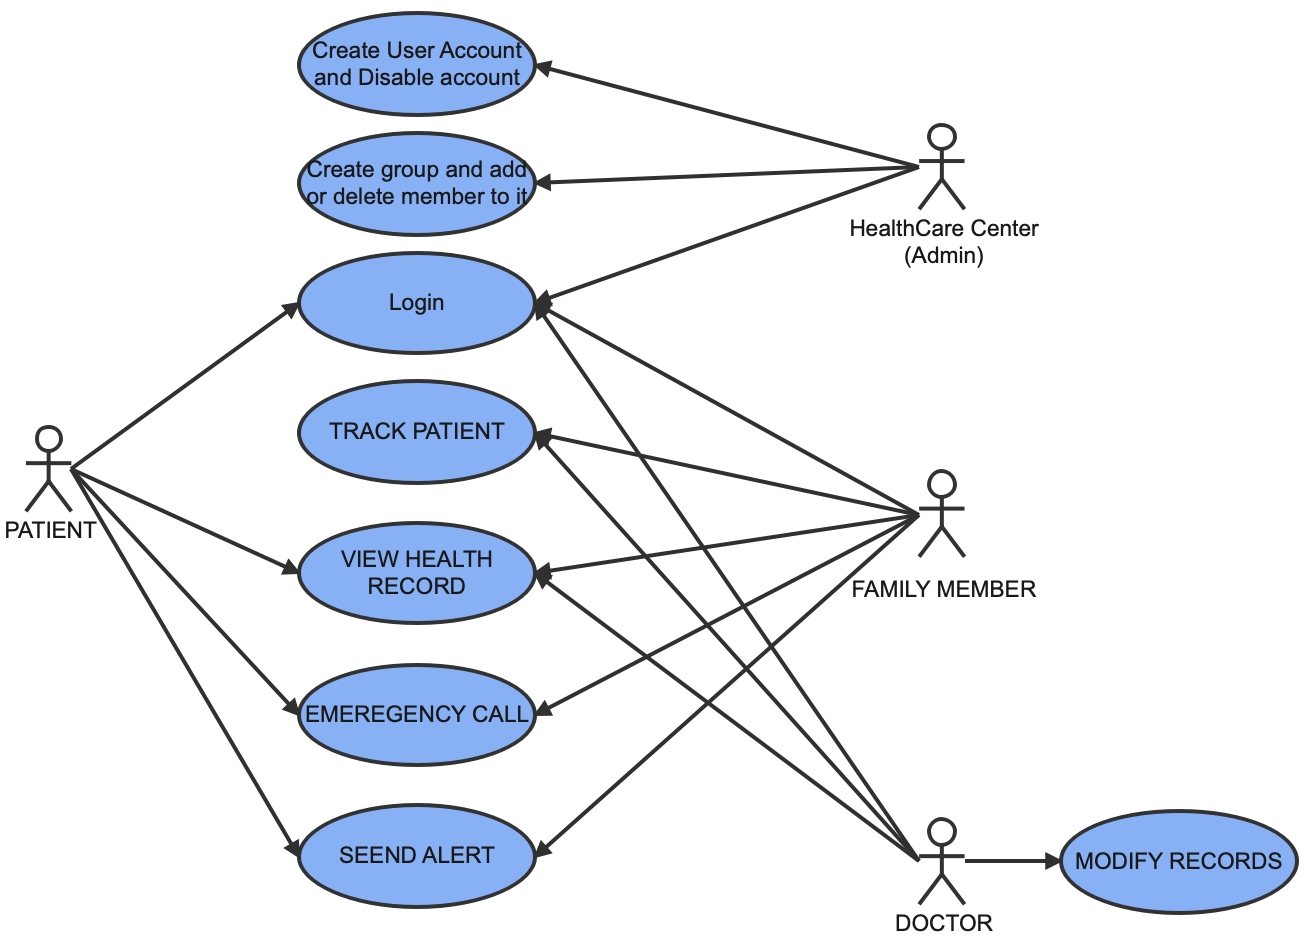
\includegraphics[width=0.8\textwidth]{use-diagram.png}
				\caption{Use Case Diagram}
				\label{Use Diagram}
			\end{figure}
			\begin{figure}[!h]
				\centering
				\includegraphics[width=\textwidth]{context-diagram.jpg}
				\caption{Context Diagram}
				\label{Context Diagram}
			\end{figure}
		\newpage
		\begin{center}
			\newpage
		\end{center}
	   
		\subsection{Functional Requirement Description}
		
			\quad Depending on the previous functional requirements, the following describes the functional requirements in more detail.
			\begin{table}[!h]
				\centering
				\caption{Functional Requirement Description}
				\begin{subtable}{\textwidth}
					\centering
					\caption{Doctor, Family member}
					\begin{tabular}{|l|p{10cm}|}
						\hline
						\rowcolor{lightgray}
						\textbf{Actor} & \textbf{Doctor, Family member} \\
						\hline
						\textbf{Description} & The family members and doctors can see the medical records of the patient \\
						\hline
						\textbf{Preconditions} & The family member allows the doctor to see their patient records by the patient ID number \\
						\hline
						\textbf{Basic processes} & The family members and doctors can follow-up of the patient's health condition and send alerts of any of them see any danger of patients life \\
						\hline
						\textbf{The exceptional} & If the patient is unconscious, some of information in the record is opened without the consent of the patient, and automatically send alerts to the doctor and the family members \\
						\hline
					\end{tabular}
				\end{subtable}
				\begin{center}
				\end{center}
				\begin{subtable}{\textwidth}
					\centering
					\caption{Patient}
					\begin{tabular}{|l|p{10cm}|}
						\hline
						\rowcolor{lightgray}
						\textbf{Actor} & \textbf{Patient} \\
						\hline
						\textbf{Description} & Patient Can See His Health Record but He Can't Edit the Record , Only The Doctor Can (Add,Delete,Edit) His Record \\
						\hline
						\textbf{Preconditions} & The Family Member Allows the Doctor to See Their Patient Records by The Patient ID Number After taking the patient's opinion \\
						\hline
						\textbf{Basic Processes} & Patient Send Alert And Open An Emergency Call If There is Any Danger On His Life And His Health , Also His Family And Doctor Track His Location And See His Health Status \\
						\hline
						\textbf{The Exceptional} & If the patient is unconscious, Some of Information in the record is opened without the consent of the patient, And Automatically Send Alerts to The Doctor And the Family Members \\
						\hline
					\end{tabular}
				\end{subtable}
			\end{table}
		\newpage
		
		
		\subsection{Summary}
		
			\quad Building the system needs the following stages, which are planning, analysis, design, implementation and maintenance, so in this chapter we analyzed and described the functional requirements, so a detailed explanation of the requirements was made, and the relationship of each requirement was determined with the elements of the system, the inputs and outputs of each of them were determined and the modeling of the system was.
			\newpage
			
			\section*{\begin{center}
					Chapter Four
			\end{center}}
			\section{SYSTEM DESIGN}
			\subsection{Introduction}
			\subsubsection{Algorithms}
			
			\quad The Advanced Encryption Standard (AES) is widely regarded as one of the best symmetric encryption algorithms currently available. Its high level of security, speed, and versatility make it a popular choice for protecting sensitive data in various industries, including healthcare. AES is frequently used to safeguard personal and medical information, among other things.
			SHA (Secure Hash Algorithm) is a family of cryptographic hash functions commonly employed to create digital signatures and authenticate data integrity.\\
			
			Encryption is the method of transforming data so that it is unreadable without the proper decryption key. Encryption is used to maintain data confidentiality during storage or transmission, ensuring that only authorized users can access it. Hashing, on the other hand, is the process of converting data into a fixed-length value or key that represents the original data. The purpose of hashing is to confirm the data's integrity and authenticity. Hashing creates a unique digital fingerprint of the data that can be used to check if the data has been tampered with or altered. In summary, encryption protects data confidentiality, while hashing verifies data integrity and authenticity.\\
			
			Both AES and SHA-256 are widely acknowledged as efficient and do not consume excessive battery power on mobile devices when appropriately implemented and optimized. However, the battery usage of any algorithm is determined by various factors such as the size of data being encrypted/hashed, the frequency of encryption/hashing, and the hardware and software specifications of the device itself.\\
			
			AES and SHA-256 are recognized as the best encryption and hashing algorithms, respectively, due to their strong security features and efficiency. They have been extensively used in many applications, including mobile devices, and have proven energy-efficient. Moreover, AES and SHA-256 are widely accepted and recommended by industry experts because they provide a high level of security and protection for sensitive data such as personal and medical information, which is critical for a patient tracker app.\\
			
			The selection of the AES and SHA-256 algorithms for the patient tracker app was based on several key factors, including their strong security features, industry standards, and proven effectiveness in protecting sensitive data.\\
			
			AES (Advanced Encryption Standard) is a symmetric encryption algorithm that has been extensively analyzed and recognized by the National Institute of Standards and Technology (NIST) as a secure and efficient encryption algorithm \cite{daemen2002design}. It offers a high level of security, ensuring that patient data remains confidential and protected from unauthorized access.\\
			
			SHA-256 (Secure Hash Algorithm) is a cryptographic hash function that belongs to the SHA-2 family. It is widely used for data integrity and authentication purposes (NIST, 2015). SHA-256 generates a fixed-length hash value for input data, making it suitable for verifying the integrity of patient data stored in the database. It helps detect any unauthorized modifications or tampering with the data.\\
			
			The choice of AES and SHA-256 is also driven by their acceptance as industry standards and their widespread adoption in various applications, including mobile devices. These algorithms have undergone rigorous testing, analysis, and scrutiny by the cryptographic community, ensuring their reliability and effectiveness in securing sensitive information \cite{tuli2013review}.\\
			
			Additionally, AES and SHA-256 are known for their efficiency and low battery consumption when implemented correctly. This is crucial for mobile devices, as it helps optimize the app's performance and ensures a seamless user experience.
			
			
			
			\subsubsection{PseudoCode}
			
			\quad The patient tracker app offers a user-friendly interface for managing patient information. Users can add, view, update, and delete patient records. The app follows a clear flow, prompting users to select options from the main menu and guiding them through the corresponding actions. It ensures accurate and organized data management, handles invalid selections, and terminates upon choosing the "Exit" option. The app simplifies the process of managing patient information, providing an efficient and user-friendly experience.
			
			\begin{itemize}
				\item Display welcome message and main menu options.
				\item Prompt the user to select an option from the main menu.
				\item If the user selects "Add patient":
				\begin{itemize}
					\item Prompt user to enter patient information.
					\item Add patient information to the patient list.
				\end{itemize}
				\item If the user selects "View patient":
				\begin{itemize}
					\item Prompt user to enter patient name or ID.
					\item Search the patient list for patient information.
					\item Display patient information.
				\end{itemize}
				\item If the user selects "Update patient":
				\begin{itemize}
					\item Prompt user to enter patient name or ID.
					\item Search the patient list for patient information.
					\item Prompt user to update patient information.
					\item Update patient information in the patient list.
				\end{itemize}
				\item If the user selects "Delete patient":
				\begin{itemize}
					\item Prompt user to enter patient name or ID.
					\item Search the patient list for patient information.
					\item Remove patient information from a patient list.
				\end{itemize}
				\item If the user selects "Exit":
				\begin{itemize}
					\item Display the exit message and terminate the program.
				\end{itemize}
				\item If the user selects an invalid option:
				\begin{itemize}
					\item Display an error message and prompt the user to select a valid option.
				\end{itemize}
				\item Repeat step 2 until the user selects "Exit".
			\end{itemize}
			
		
			\subsection{Class Diagram}
			\begin{figure}[!h]
				\centering
				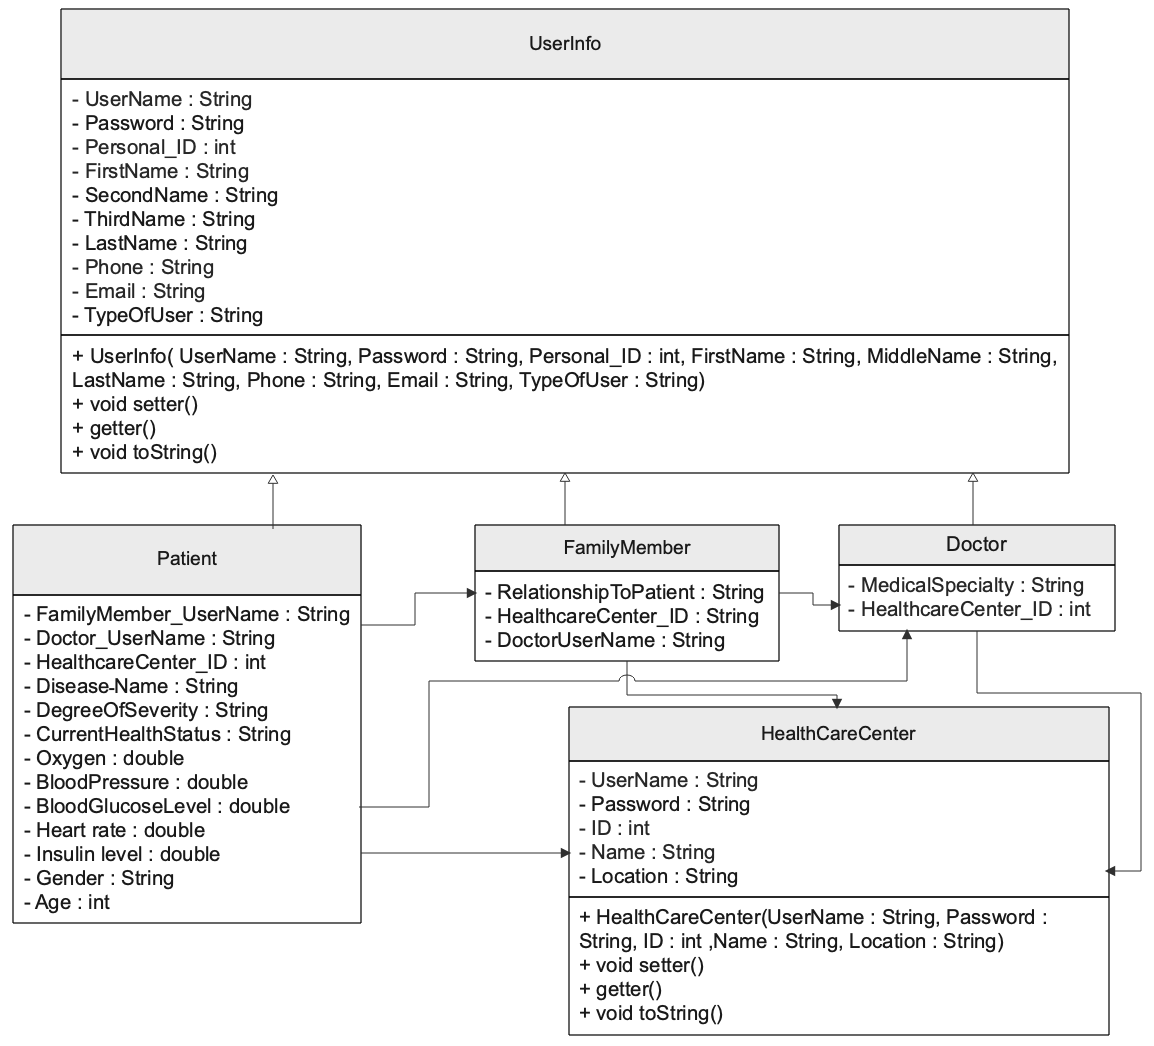
\includegraphics[width=\textwidth]{ClassDiagram.png}
				\caption{Class Diagram}
				\label{Class Diagram}
			\end{figure}
		
		\newpage
		
			\subsection{Sequence Diagrams}
			\begin{figure}[!h]
				\centering
				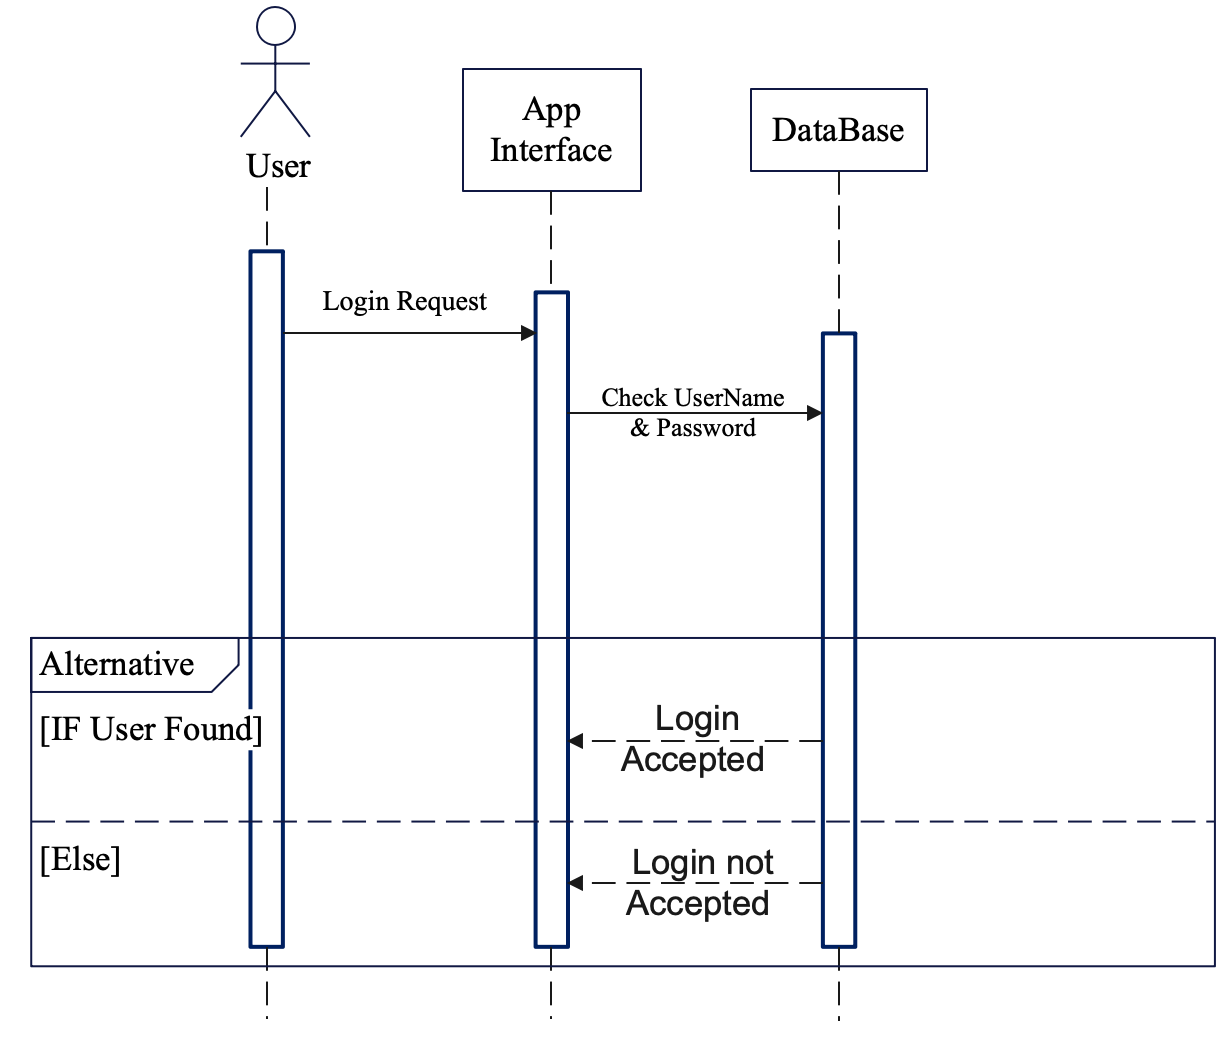
\includegraphics[width=\textwidth]{sequanceDiagram.png}
				\caption{Sequence Diagram}
				\label{Sequence Diagram}
			\end{figure}
		
		\newpage
		
			\subsection{Entity Relationship Diagram (ERD)}
				\begin{figure}[!h]
				\centering
				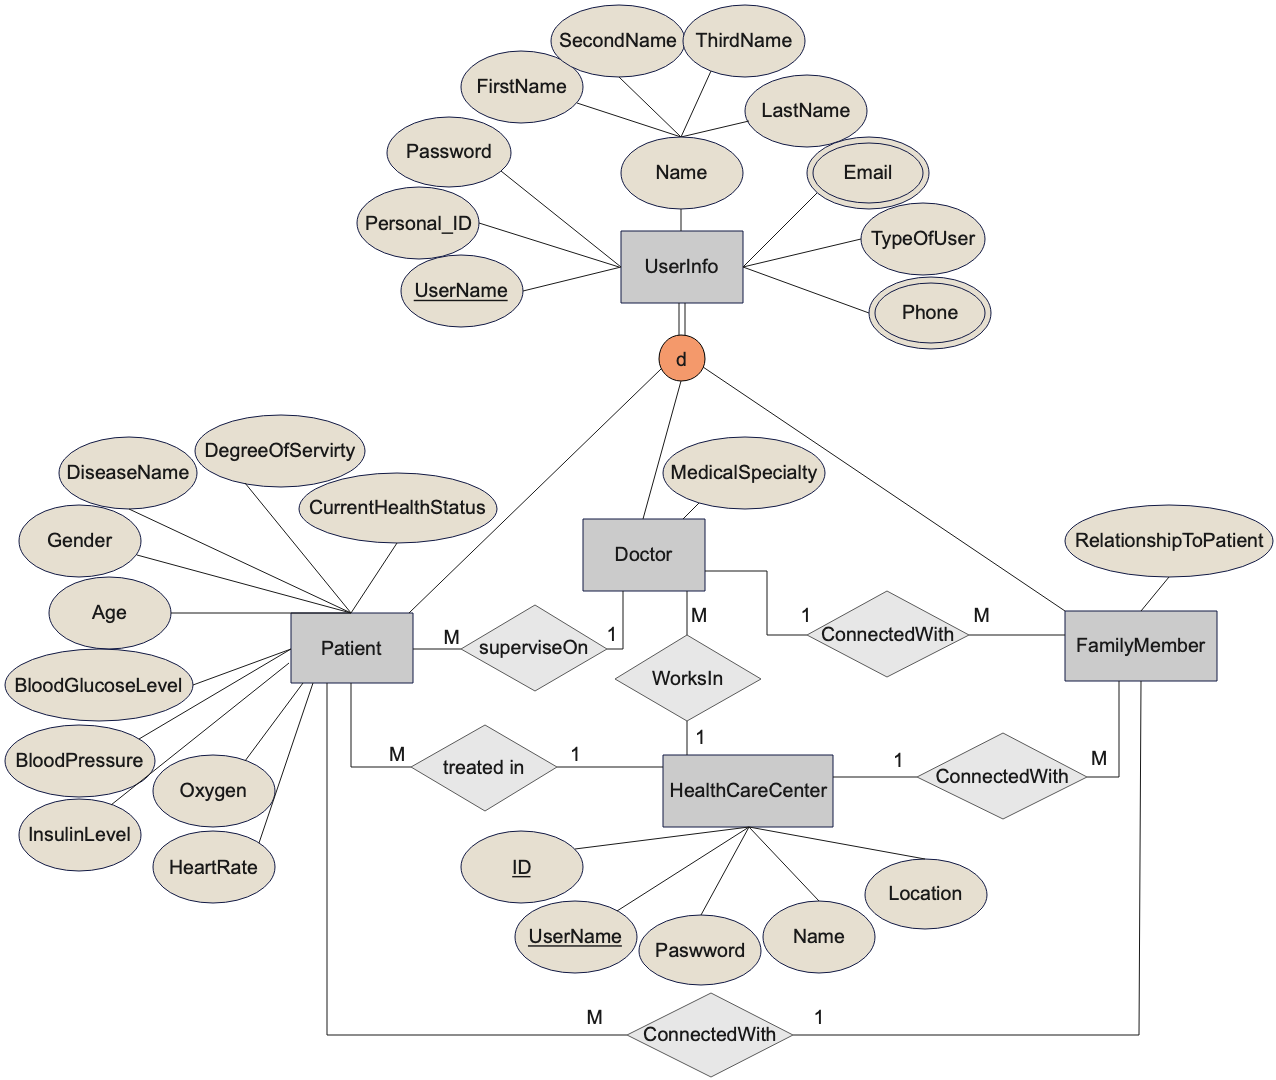
\includegraphics[width=\textwidth]{ERD.png}
				\caption{Entity Relationship Diagram (ERD)}
				\label{Entity Relationship Diagram (ERD)}
			\end{figure}
		
		\newpage
		
			\subsection{Functions Design and Activity Diagrams}
			\textbf{Functions Design :}
			\begin{itemize}
				\item User authentication and registration.
				\item Secure storage and transmission of user data.
				\item Collection and storage of user's health status information.
				\item Real-time tracking of user's location.
				\item Integration with external databases and APIs for medical data and services.
				\item Visualization of user data on a dashboard.
				\item Alerting users and medical professionals in case of critical changes in users’ health status.
				
			\end{itemize}
		
			\textbf{Activity Diagrams :}
			\begin{figure}[!h]
				\centering
				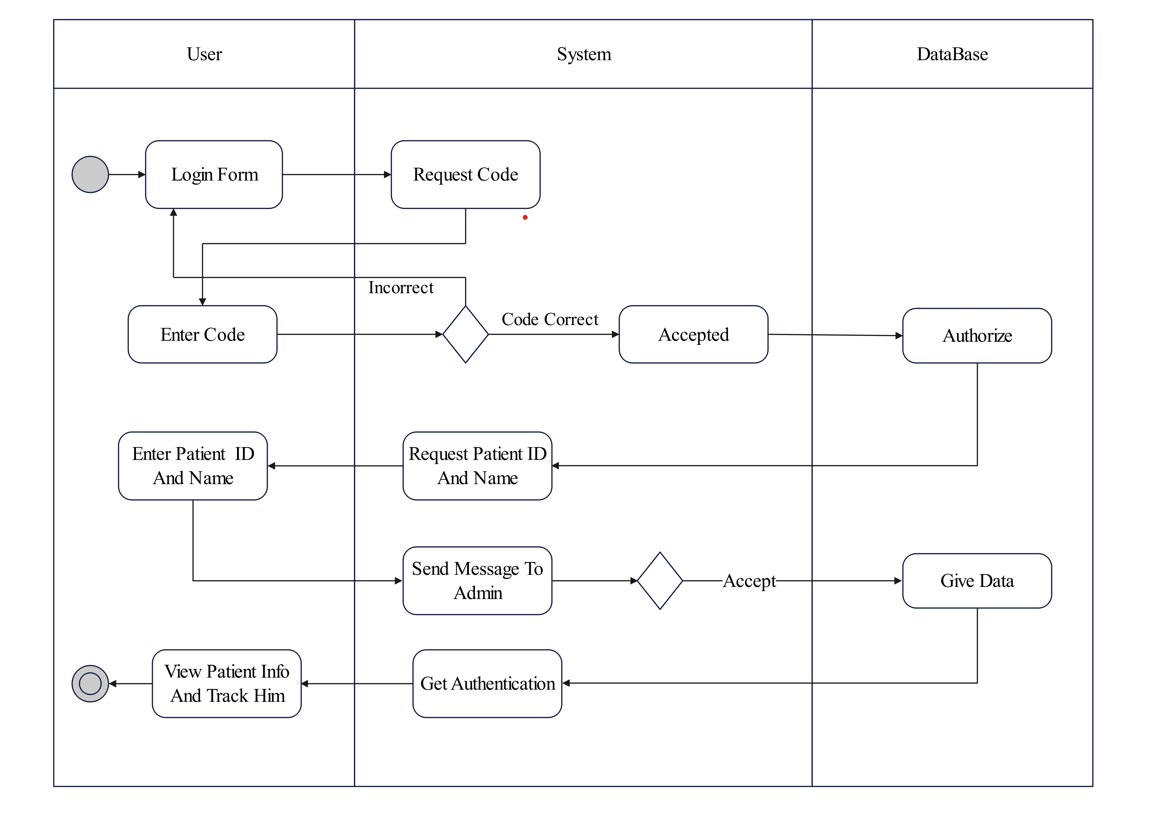
\includegraphics[width=0.8\textwidth]{Activity.png}
				\caption{Activity Diagrams}
				\label{Activity Diagrams}
			\end{figure}
			\subsection{Input/ Output Design}
			\textbf{Input :}
			\begin{itemize}
				\item User login credentials (username, password, or fingerprint).
				\item User registration information (name, email, password, city, gender, etc.).
				\item User's health status information (symptoms, vital signs(?), test results, etc.).
				\item User's location information (GPS coordinates).
				\item User's personal information (name, date of birth, etc.).
				\item User's medical history (past illnesses, medications, allergies, etc.).
				
			\end{itemize}
			\textbf{Outputs :}
			\begin{itemize}
				\item User login status (successful or unsuccessful).
				\item User registration status (successful or unsuccessful).
				\item User's health status (symptoms, vital signs, test results, etc.).
				\item User's location on a map.
				\item Alerts or notifications for critical changes in the user's health status.
				\item User's personal information.
				\item User's medical history.
				
			\end{itemize}
			\subsection{Summary}
			\quad The AES and SHA-256 encryption algorithms are secure for patient tracker apps developed using Flutter with packages like firebase\_auth, cloud\_firestore, location, and crypto. The app inputs user login, registration, health and location data, personal information, and medical history. The app outputs the user's status, health, and location information, and its functionality includes authentication, secure storage, data tracking, visualization, and alerts for critical health changes.
			
			
			\section*{\begin{center}
					Chapter Five
			\end{center}}
			
			\section{SYSTEM DEVELOPMENT}
			\subsection{Introduction}
			
			\quad The patient tracker system plays a crucial role in modern healthcare by enabling effective
			monitoring and management of patient information. System development for a patient
			tracker system involves the design, development, and implementation of software
			solutions tailored to the specific needs of healthcare organizations. It aims to provide
			healthcare professionals with a reliable and efficient platform to track and record patient
			data, facilitate communication between healthcare providers, and improve overall patient
			care.
			
			System development for a patient tracker system requires a thorough understanding of
			healthcare processes, data privacy regulations, and the unique requirements of different
			healthcare settings. It involves creating intuitive user interfaces, integrating with existing
			healthcare systems, and ensuring data accuracy and security.
			The development process includes stages such as requirements analysis, system design,
			software development, testing, and deployment. Collaboration between healthcare
			professionals, software developers, and system administrators is essential to ensure that
			the patient tracker system meets the needs of all stakeholders and aligns with industry
			standards and regulations.
			
			By implementing an effective patient tracker system, healthcare organizations can
			enhance patient outcomes, streamline administrative tasks, and improve communication
			and collaboration among healthcare providers. System development plays a vital role in
			ensuring the successful implementation and utilization of patient tracker systems in the
			healthcare industry.
			\newpage
			\subsection{User Interfaces}
			
			\quad \textbf{\underline{Launch icon and launch screen:}}
			
			\begin{figure}[!htb]
				\begin{minipage}{0.48\textwidth}
					\centering
					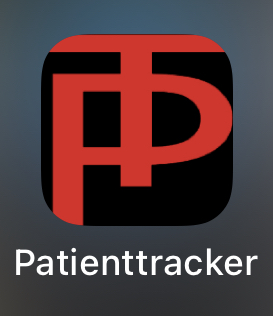
\includegraphics[width=.5\linewidth]{launchIcon.jpg}
					\caption{Launch icon}\label{Launch icon}
				\end{minipage}\hfill
				\begin{minipage}{0.48\textwidth}
					\centering
					
\includegraphics[width=.4\linewidth]{launchScreen.png}
					\caption{launch screen}\label{launch screen}
				\end{minipage}
			\end{figure}
		
			\textbf{Sign in Screen:}
				\begin{figure}[!h]
					\centering
					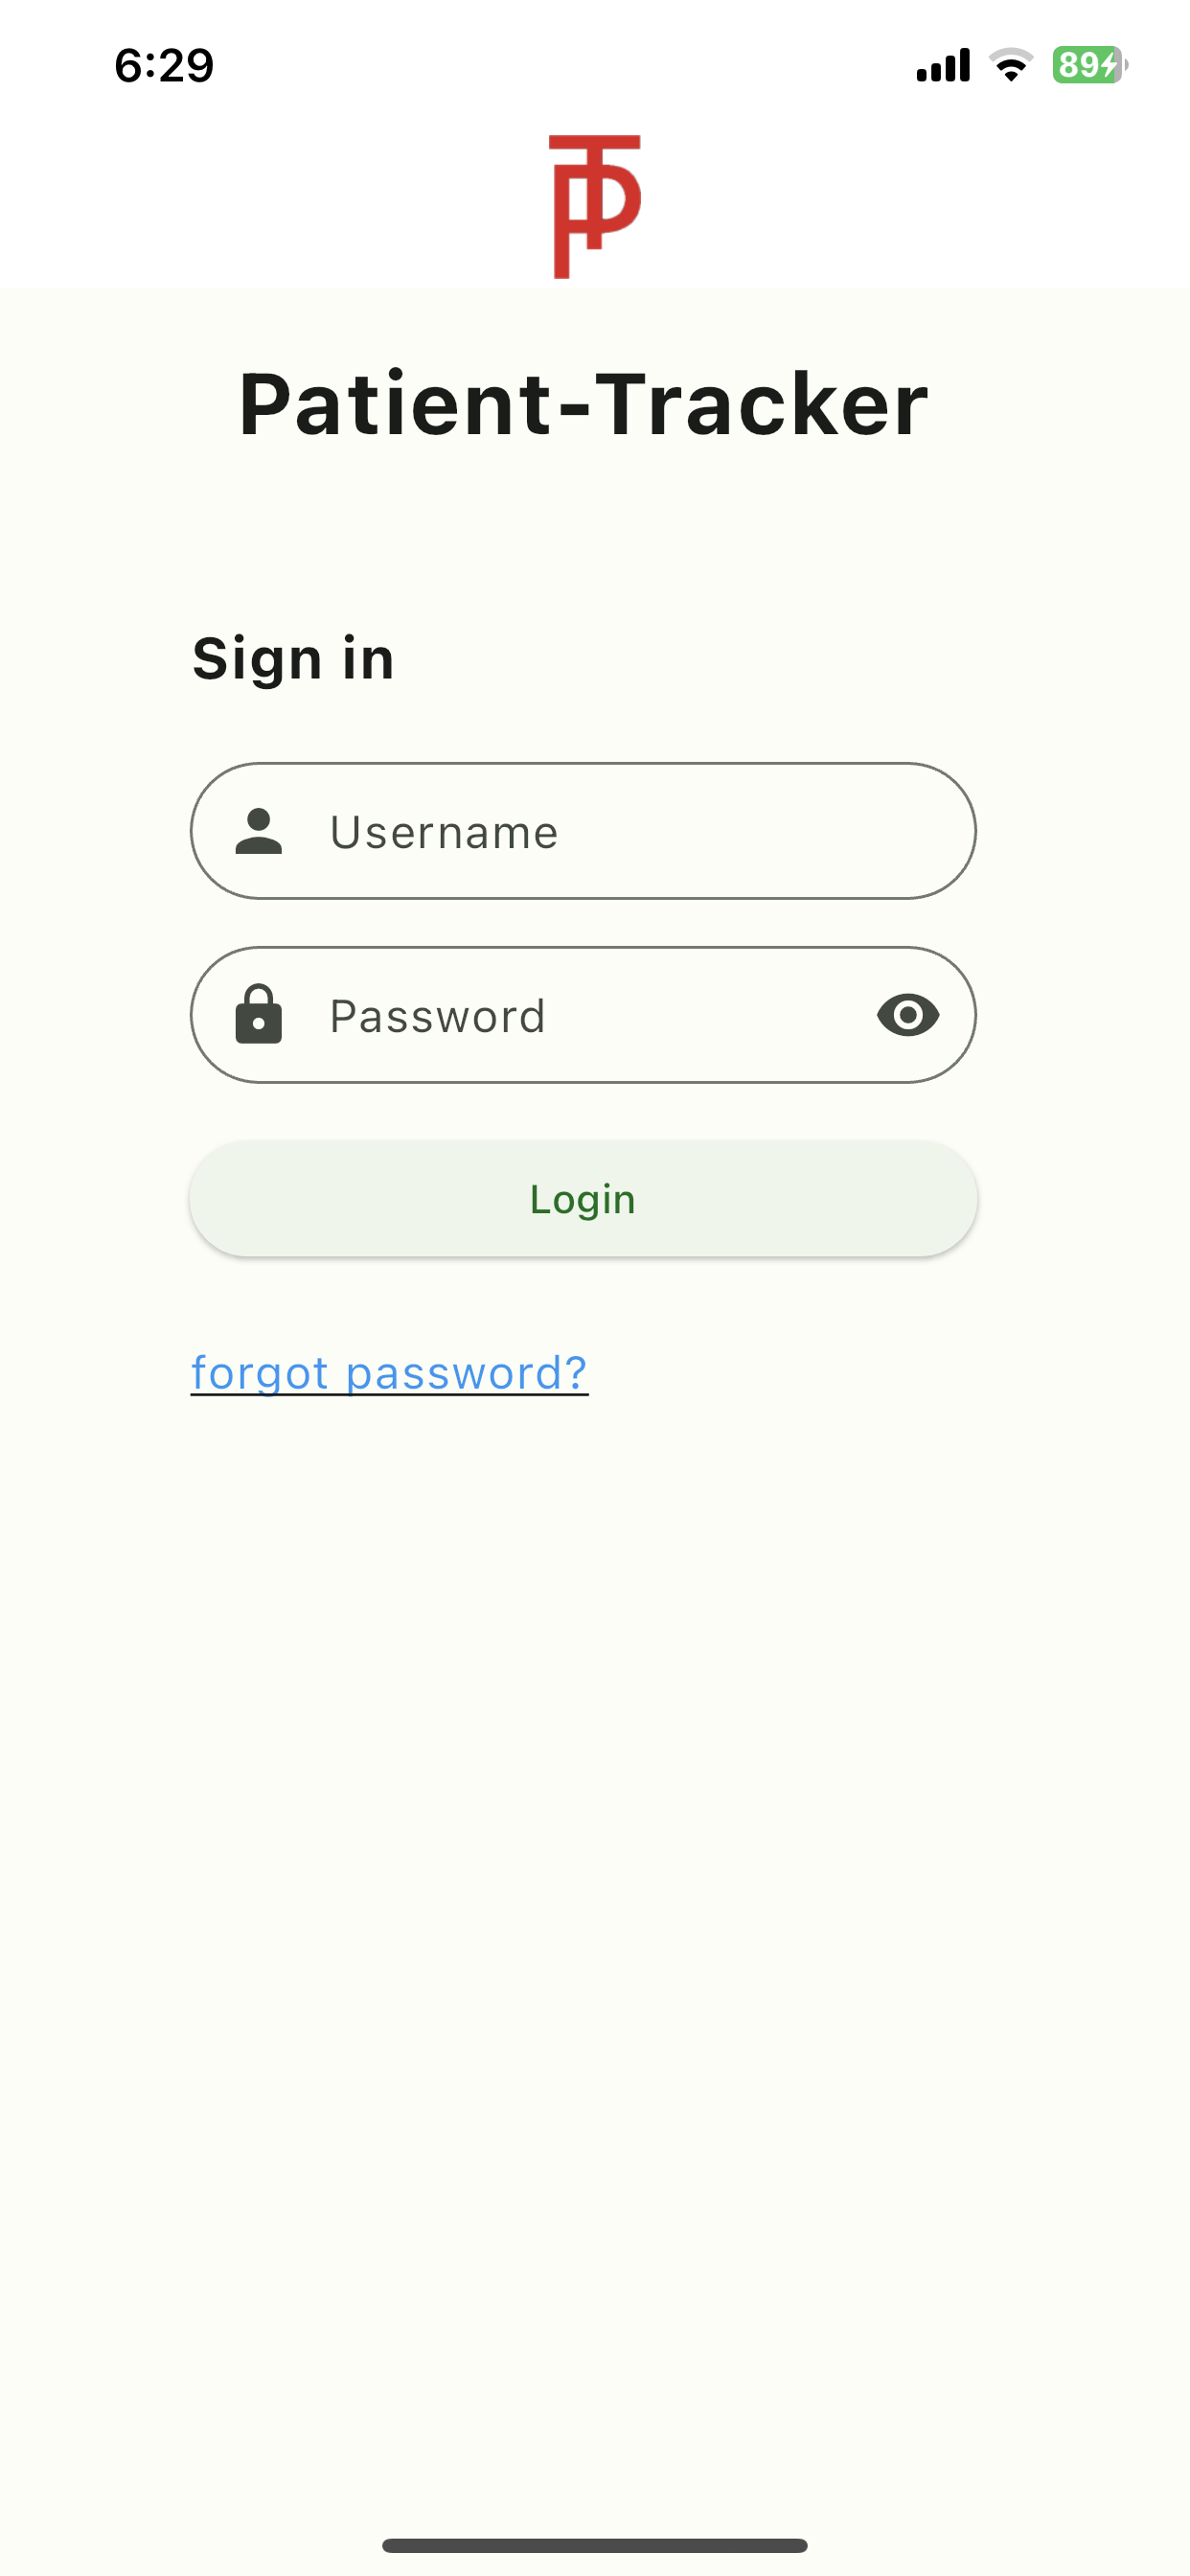
\includegraphics[width=0.25\textwidth]{SignIn.png}
					\caption{Sign in screen}
					\label{Sign in  screen}
				\end{figure}
			\newpage
		\textbf{\underline{HealthCare center screens:}}
		\begin{figure}[!htb]
			\begin{minipage}{0.48\textwidth}
				\centering
				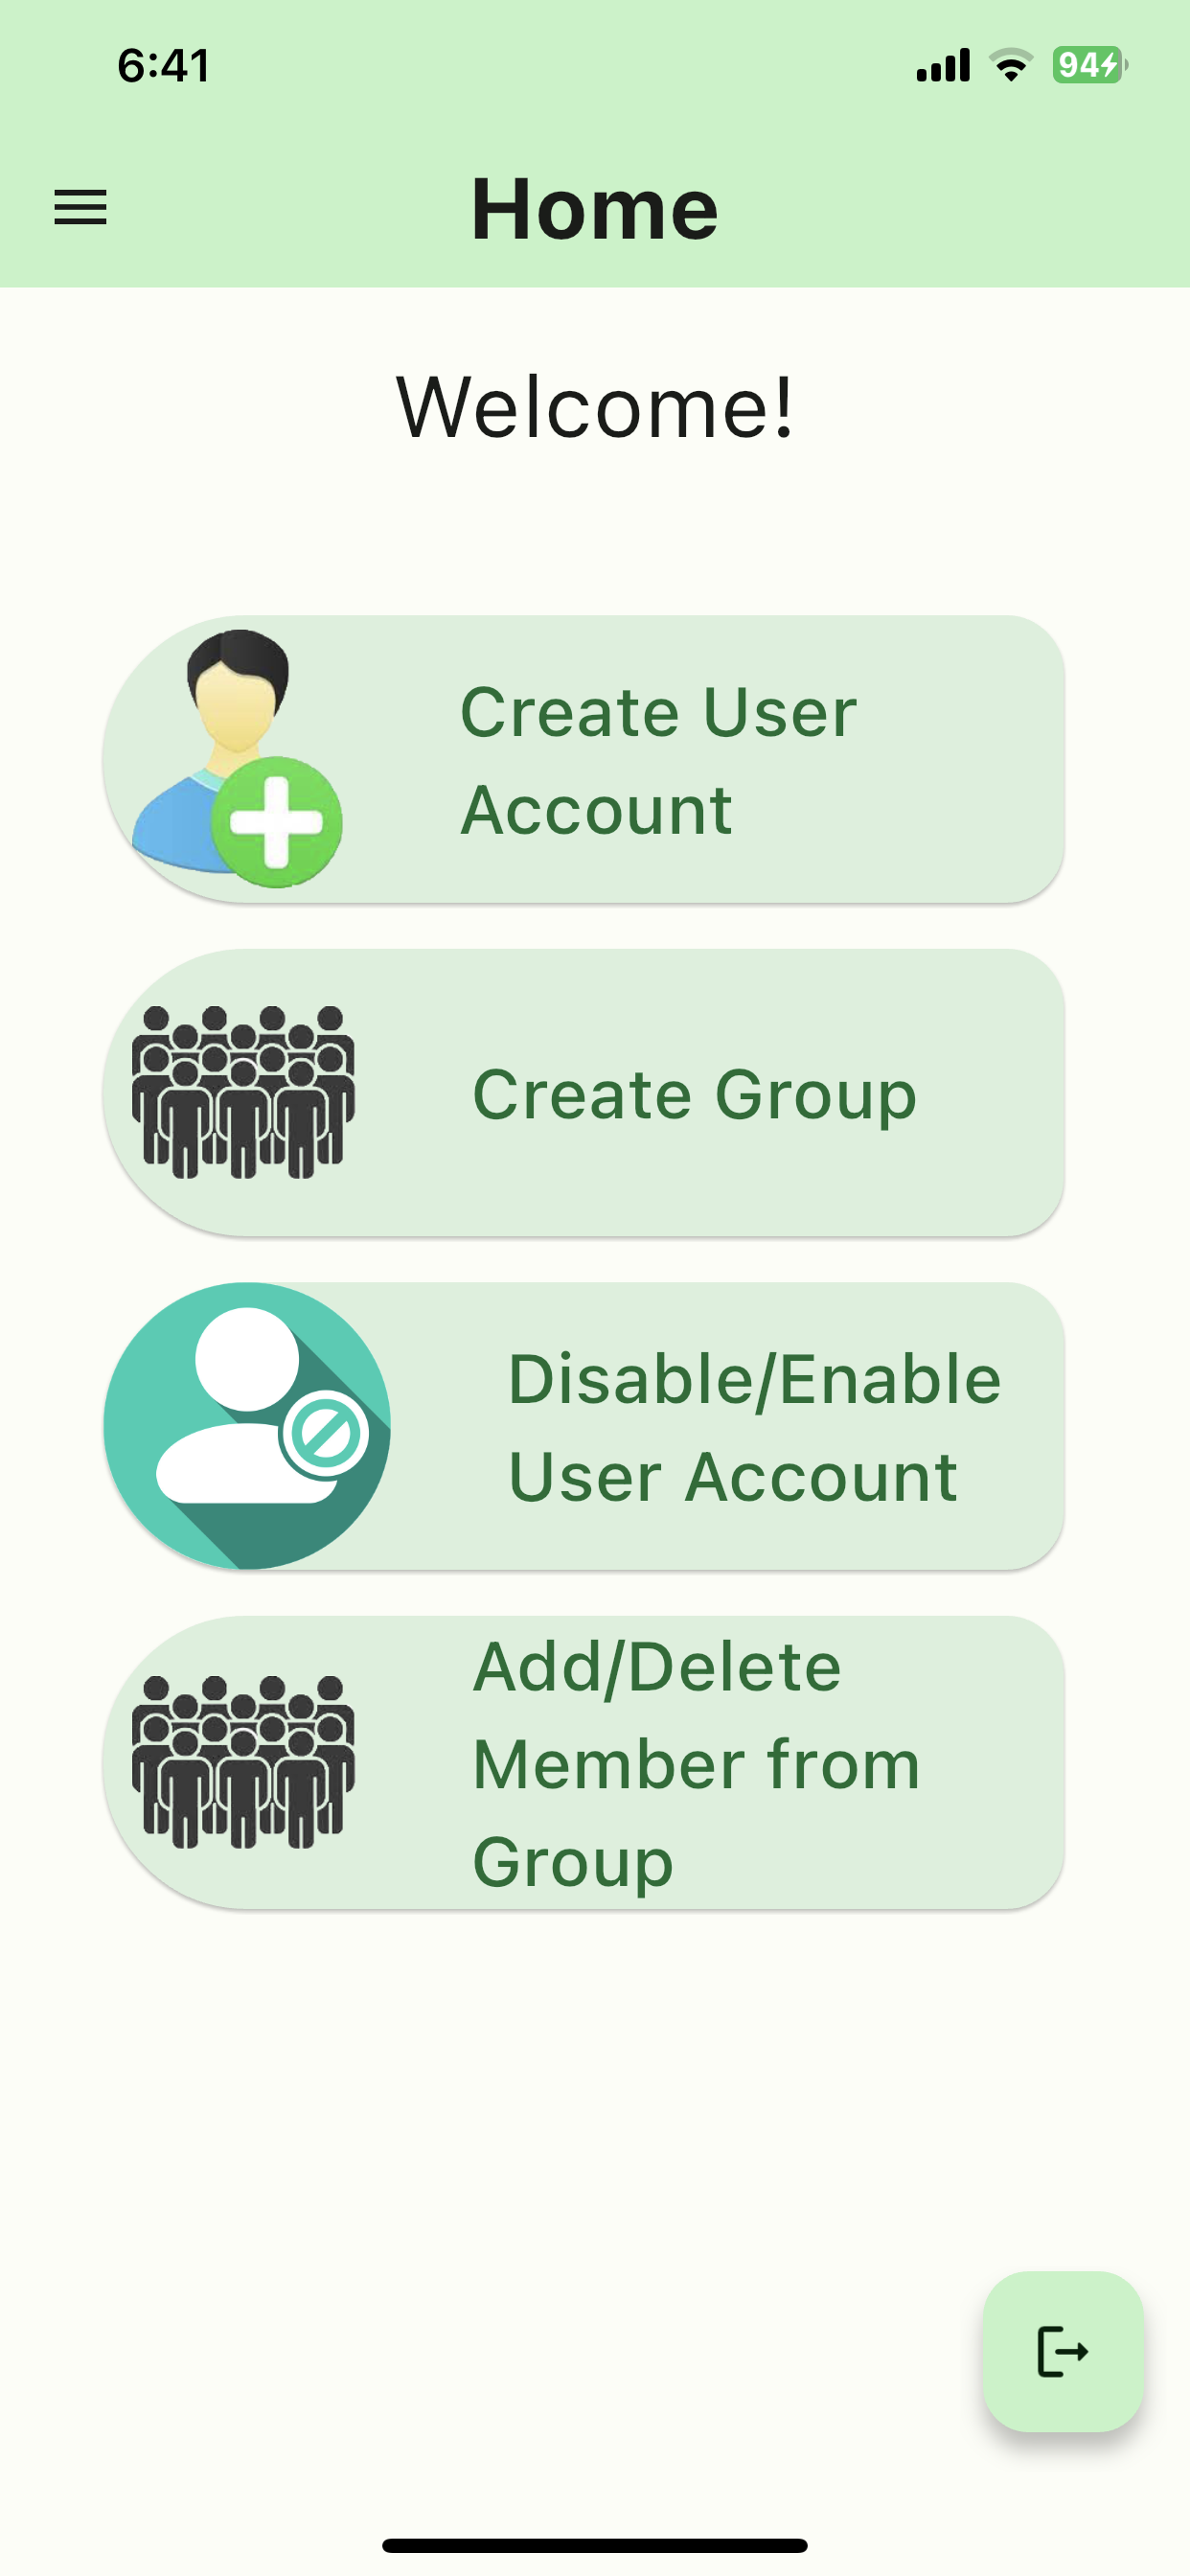
\includegraphics[width=.5\linewidth]{healthCareCenterHome.png}
				\caption{healthCare Center Home}\label{healthCare Center Home}
			\end{minipage}\hfill
			\begin{minipage}{0.48\textwidth}
				\centering
				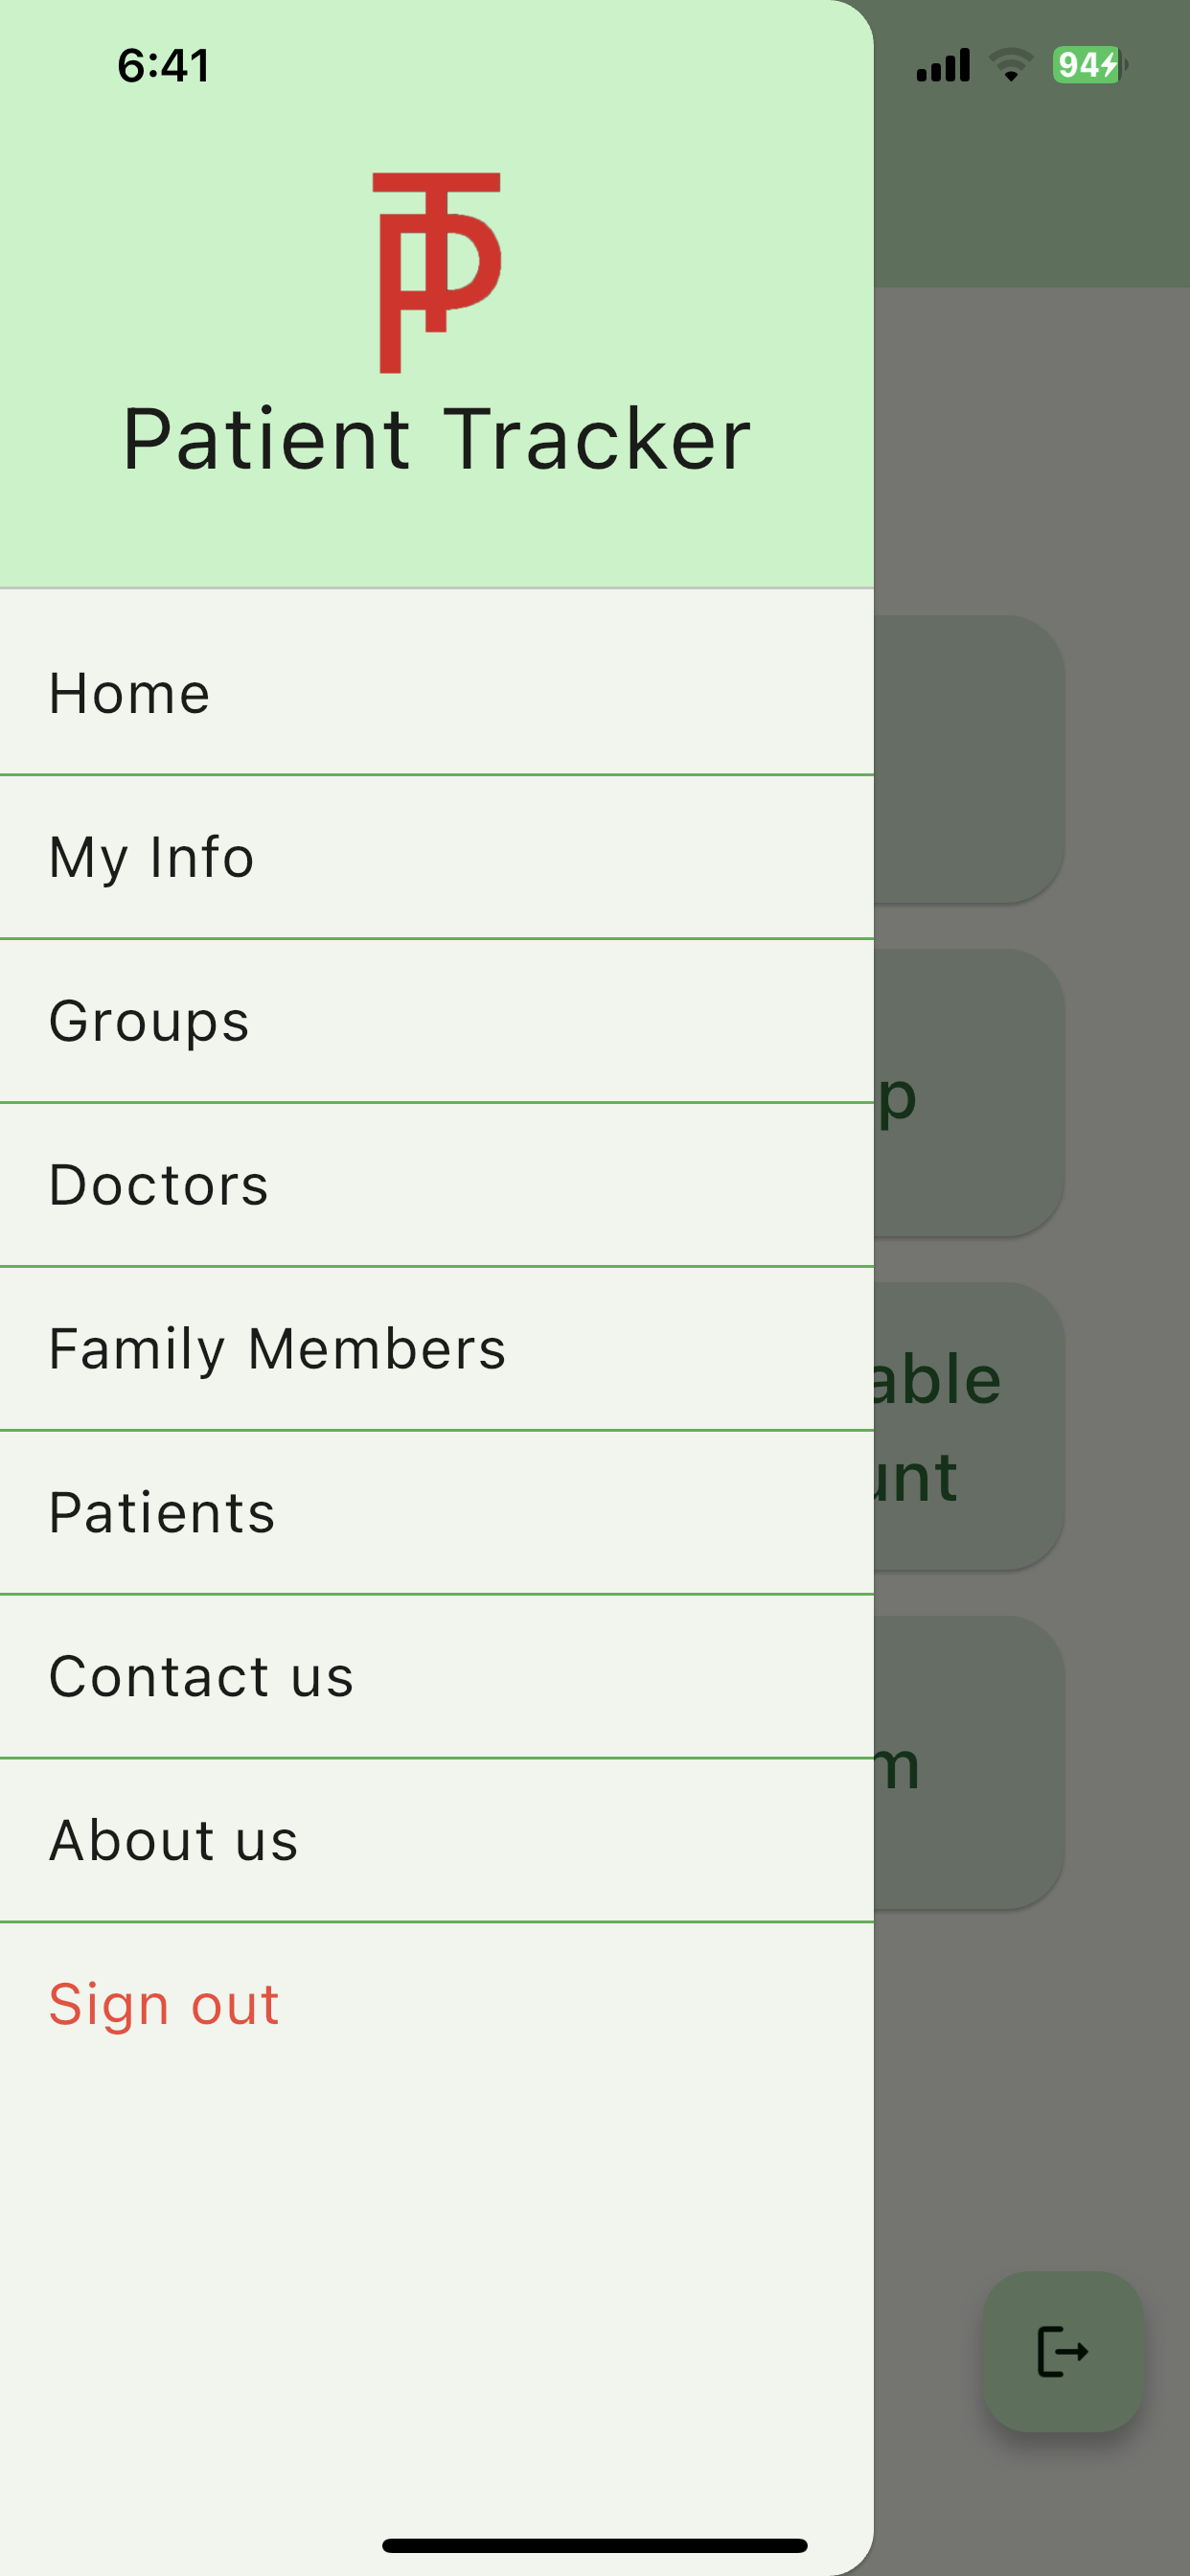
\includegraphics[width=.5\linewidth]{DrawerHealthCare.png}
				\caption{Drawer HealthCare}\label{Drawer HealthCare}
			\end{minipage}
		\end{figure}
	
		\begin{figure}[!htb]
		\begin{minipage}{0.48\textwidth}
			\centering
			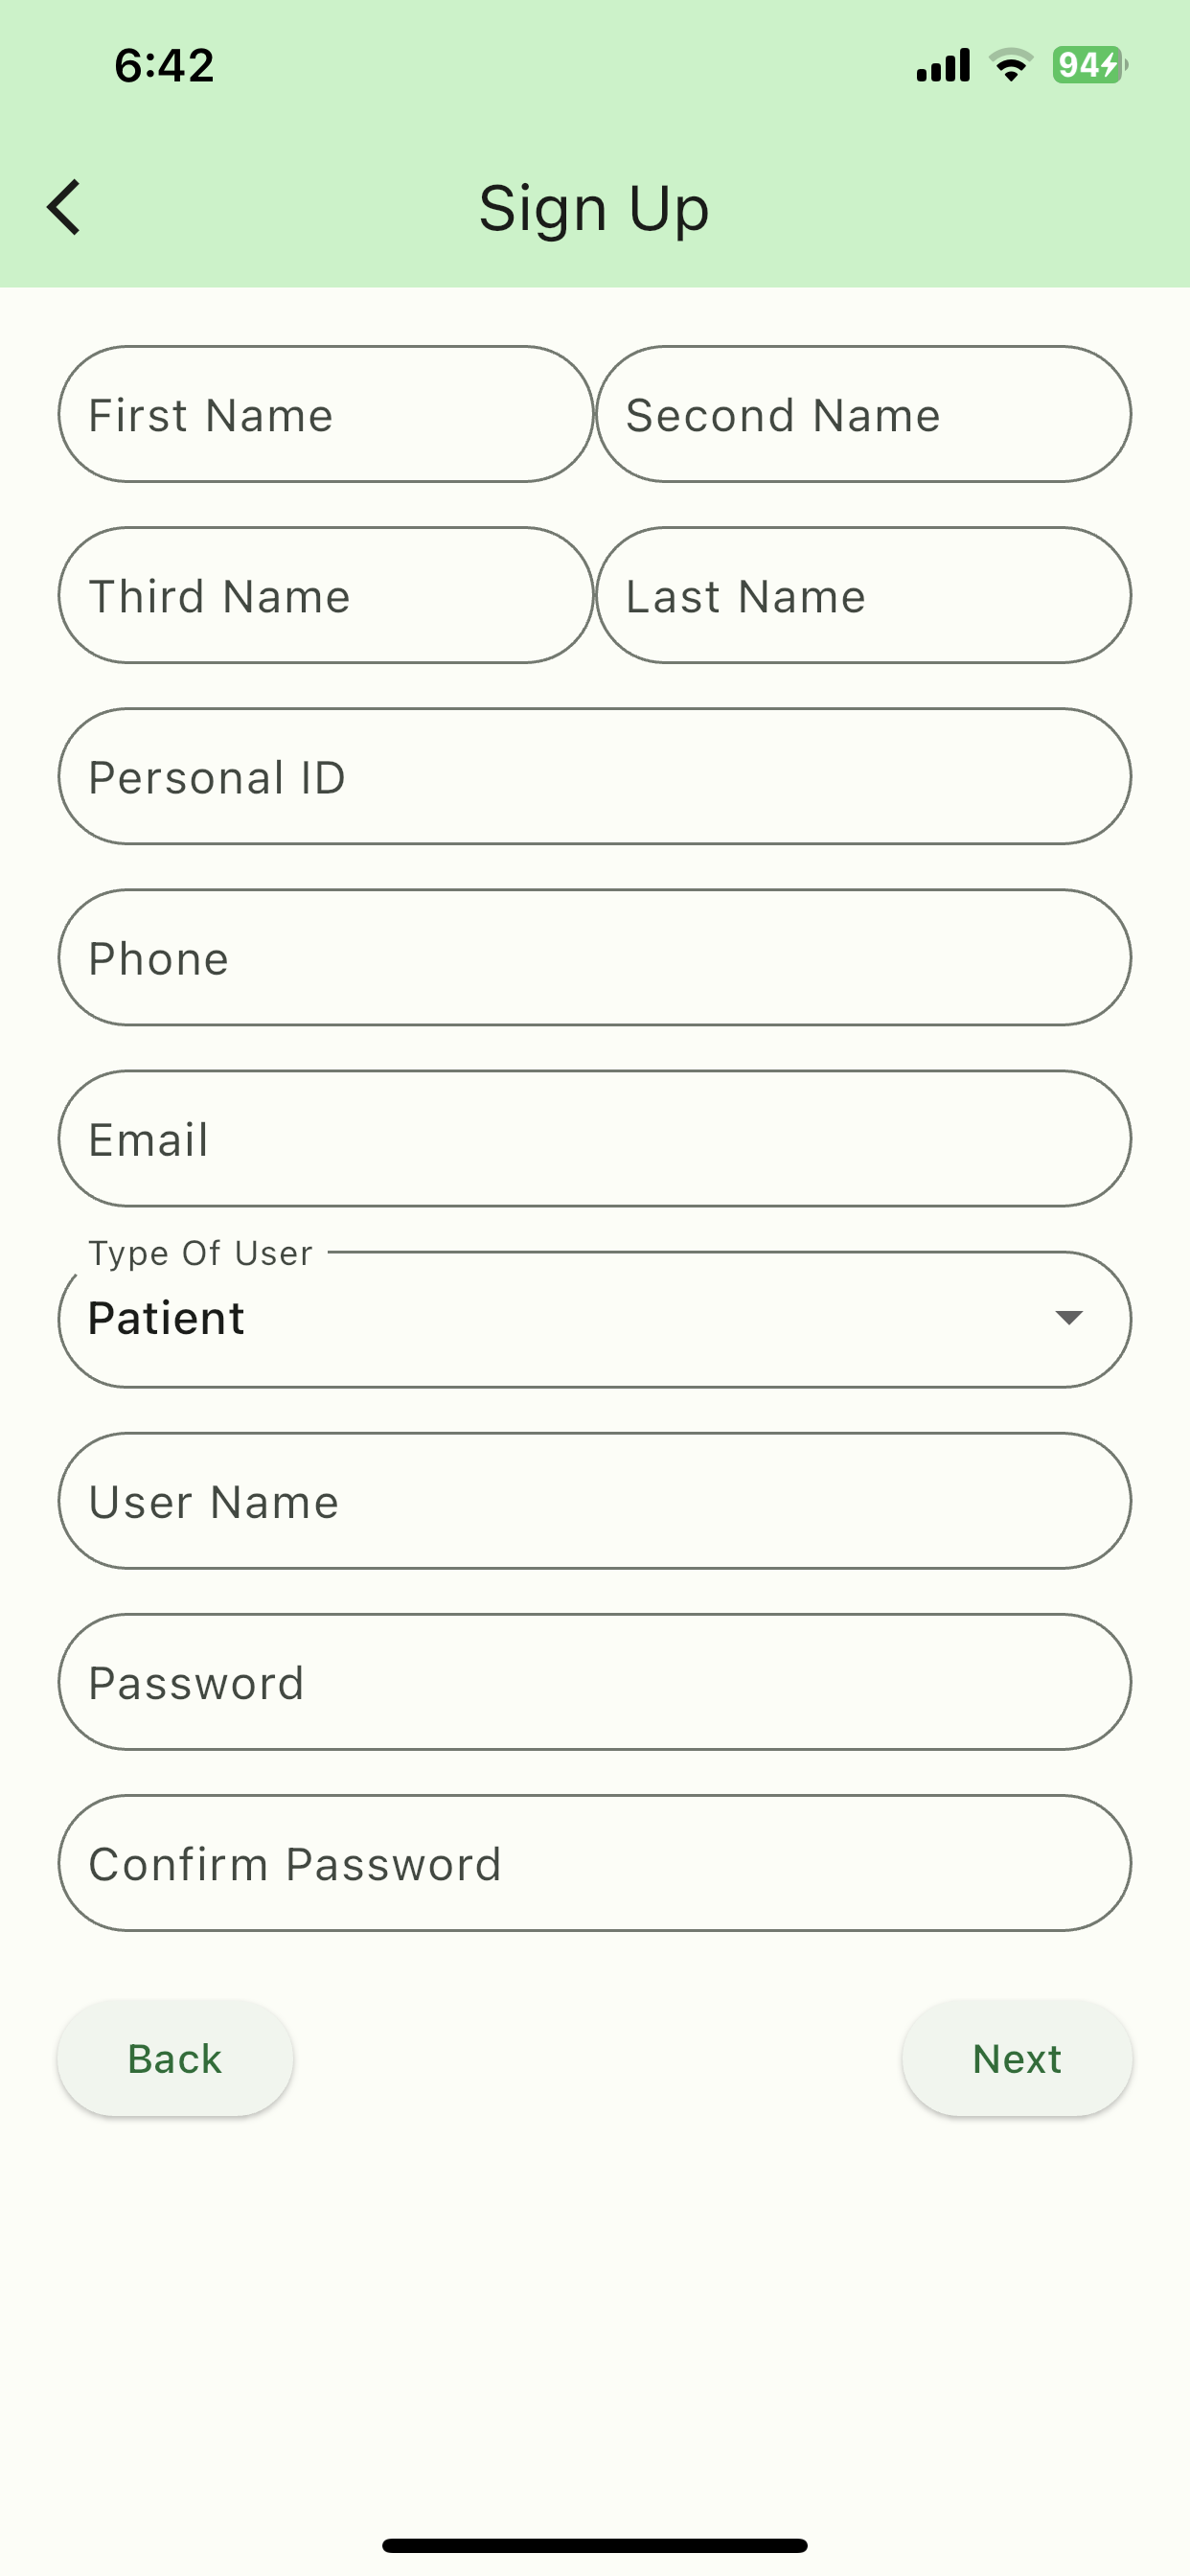
\includegraphics[width=.5\linewidth]{SignUpUser.png}
			\caption{SignUp User}\label{SignUp User}
		\end{minipage}\hfill
		\begin{minipage}{0.48\textwidth}
			\centering
			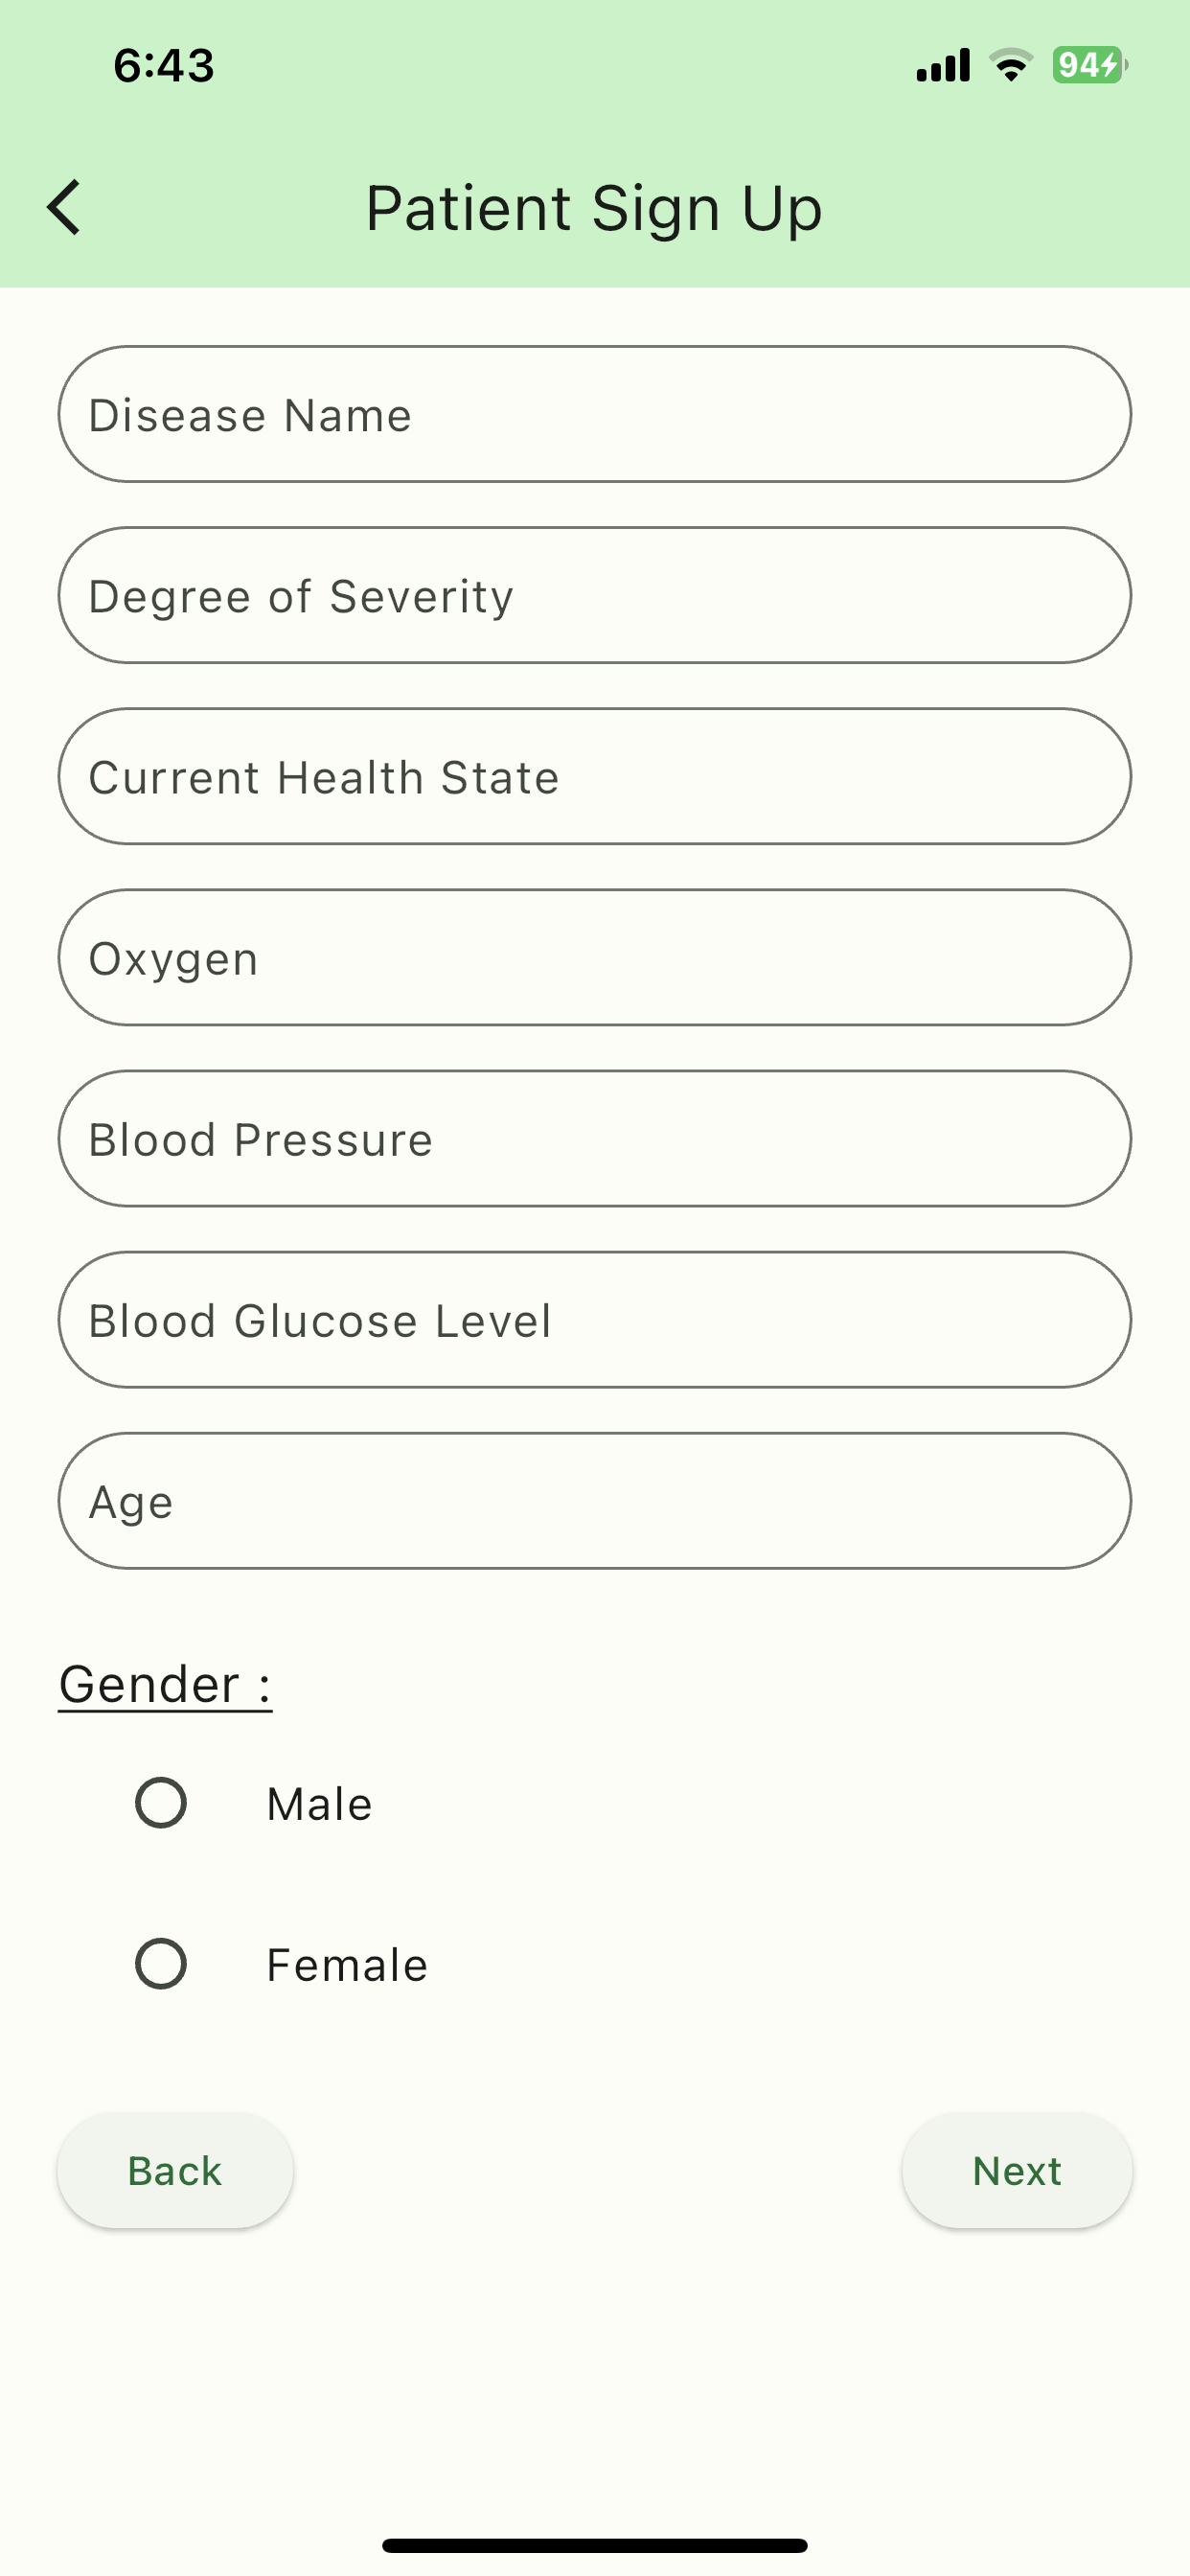
\includegraphics[width=.5\linewidth]{signUpPatient1.png}
			\caption{signUp Patient-1}\label{signUp Patient_1}
		\end{minipage}
	\end{figure}
\newpage
	\begin{figure}[!htb]
	\begin{minipage}{0.48\textwidth}
		\centering
		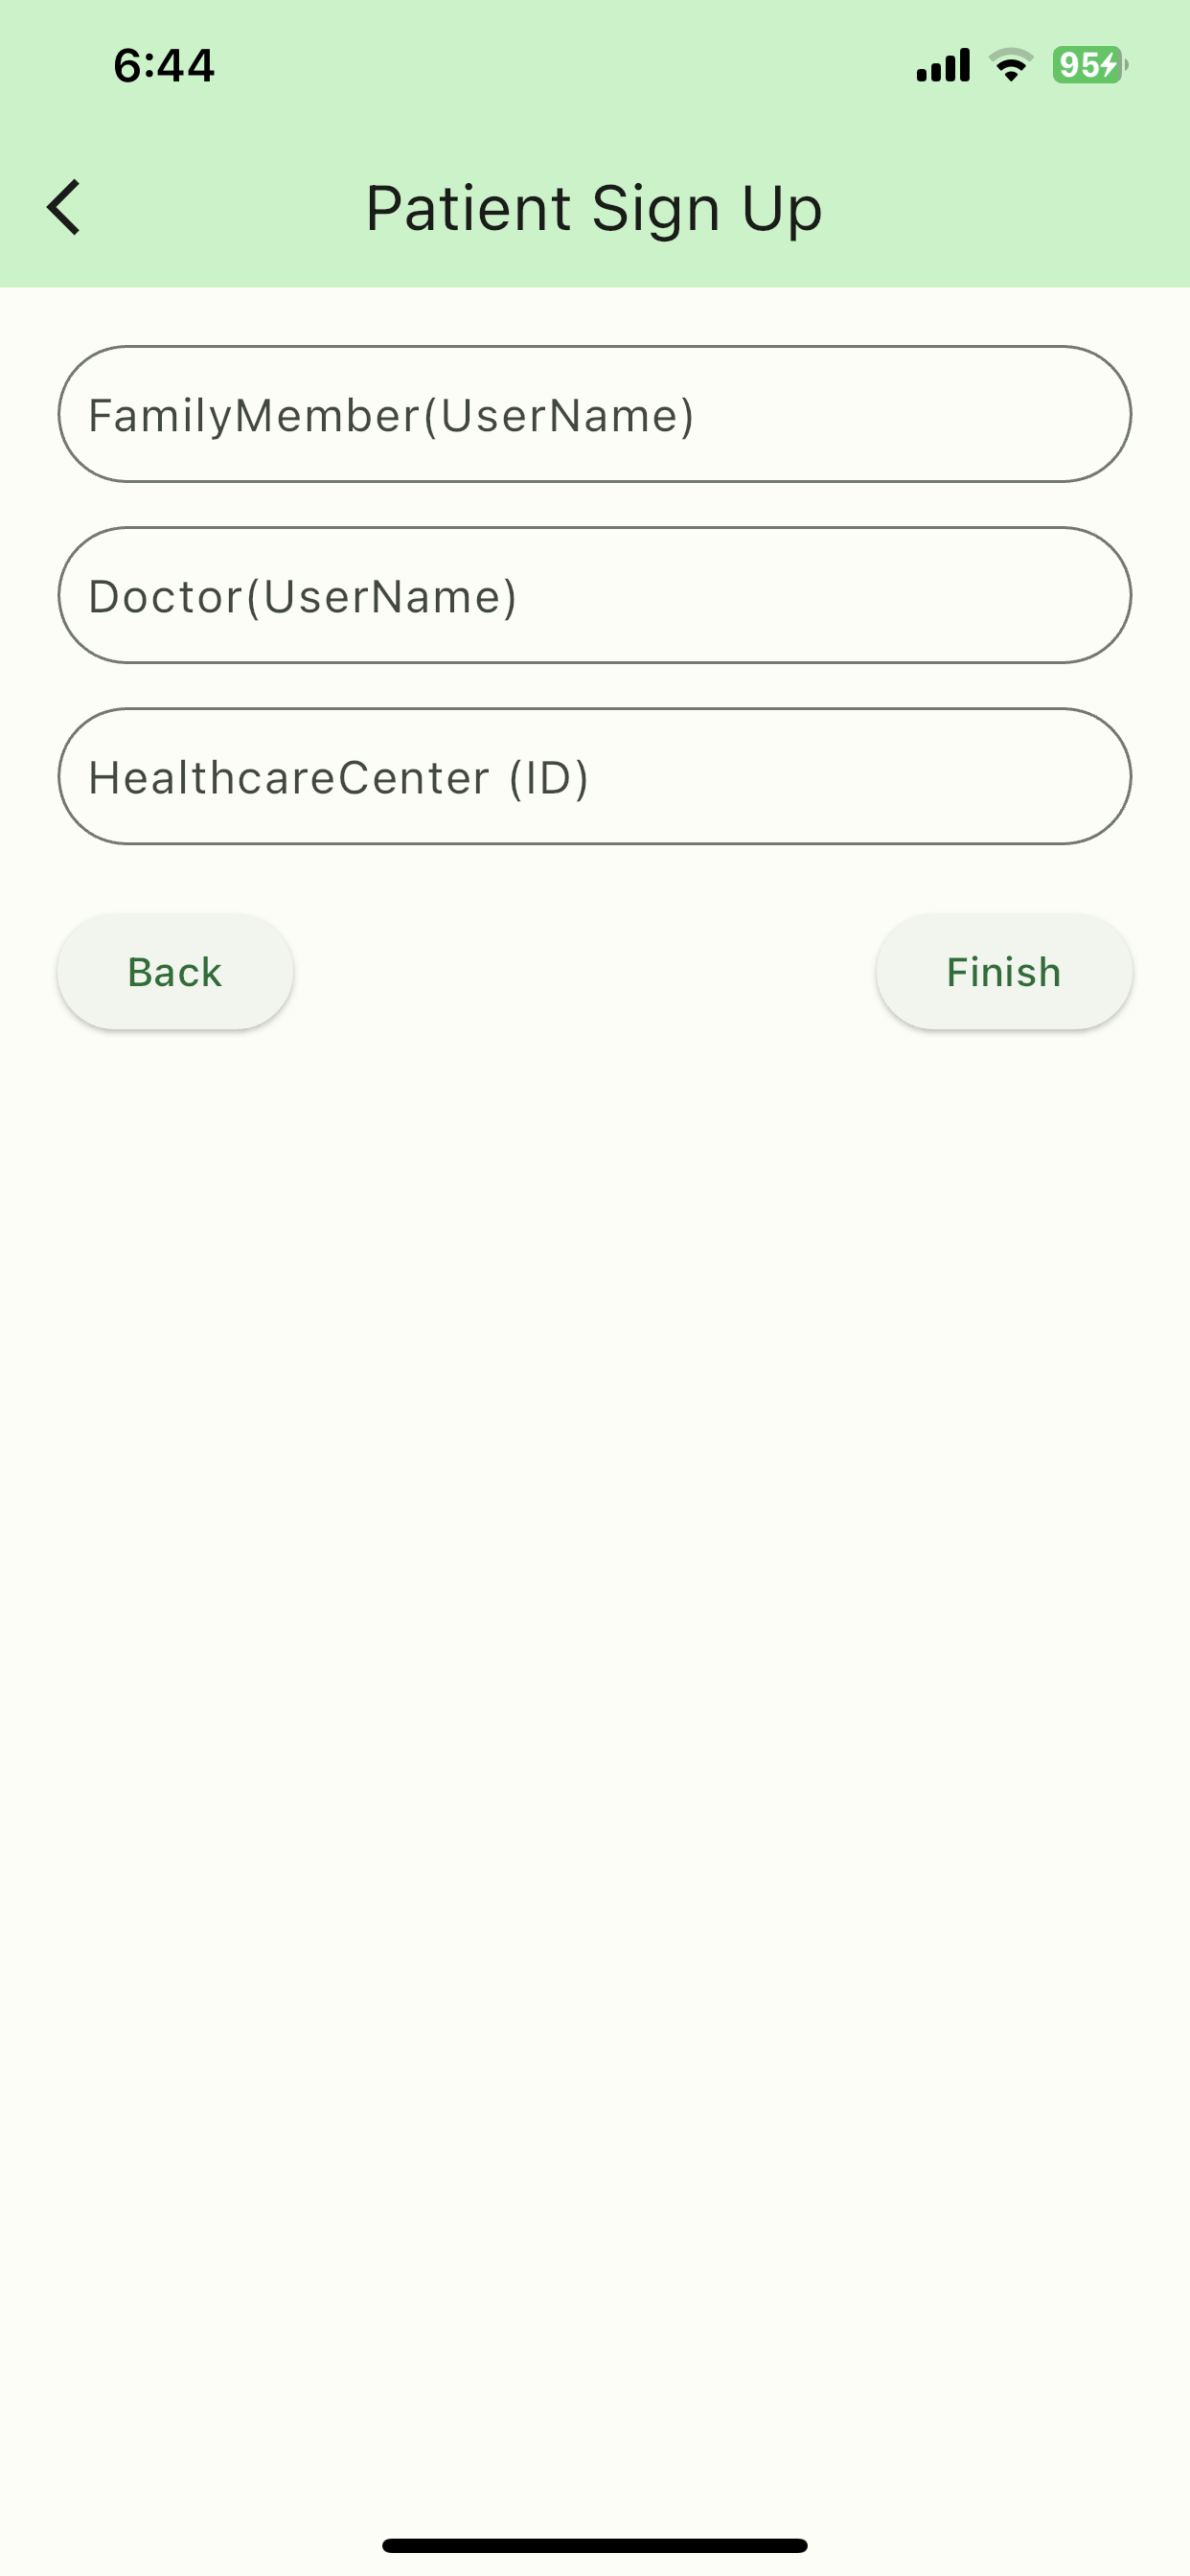
\includegraphics[width=.5\linewidth]{SignUpPatient2.png}
		\caption{SignUp Patient-2}\label{SignUp Patient_2}
	\end{minipage}\hfill
	\begin{minipage}{0.48\textwidth}
		\centering
		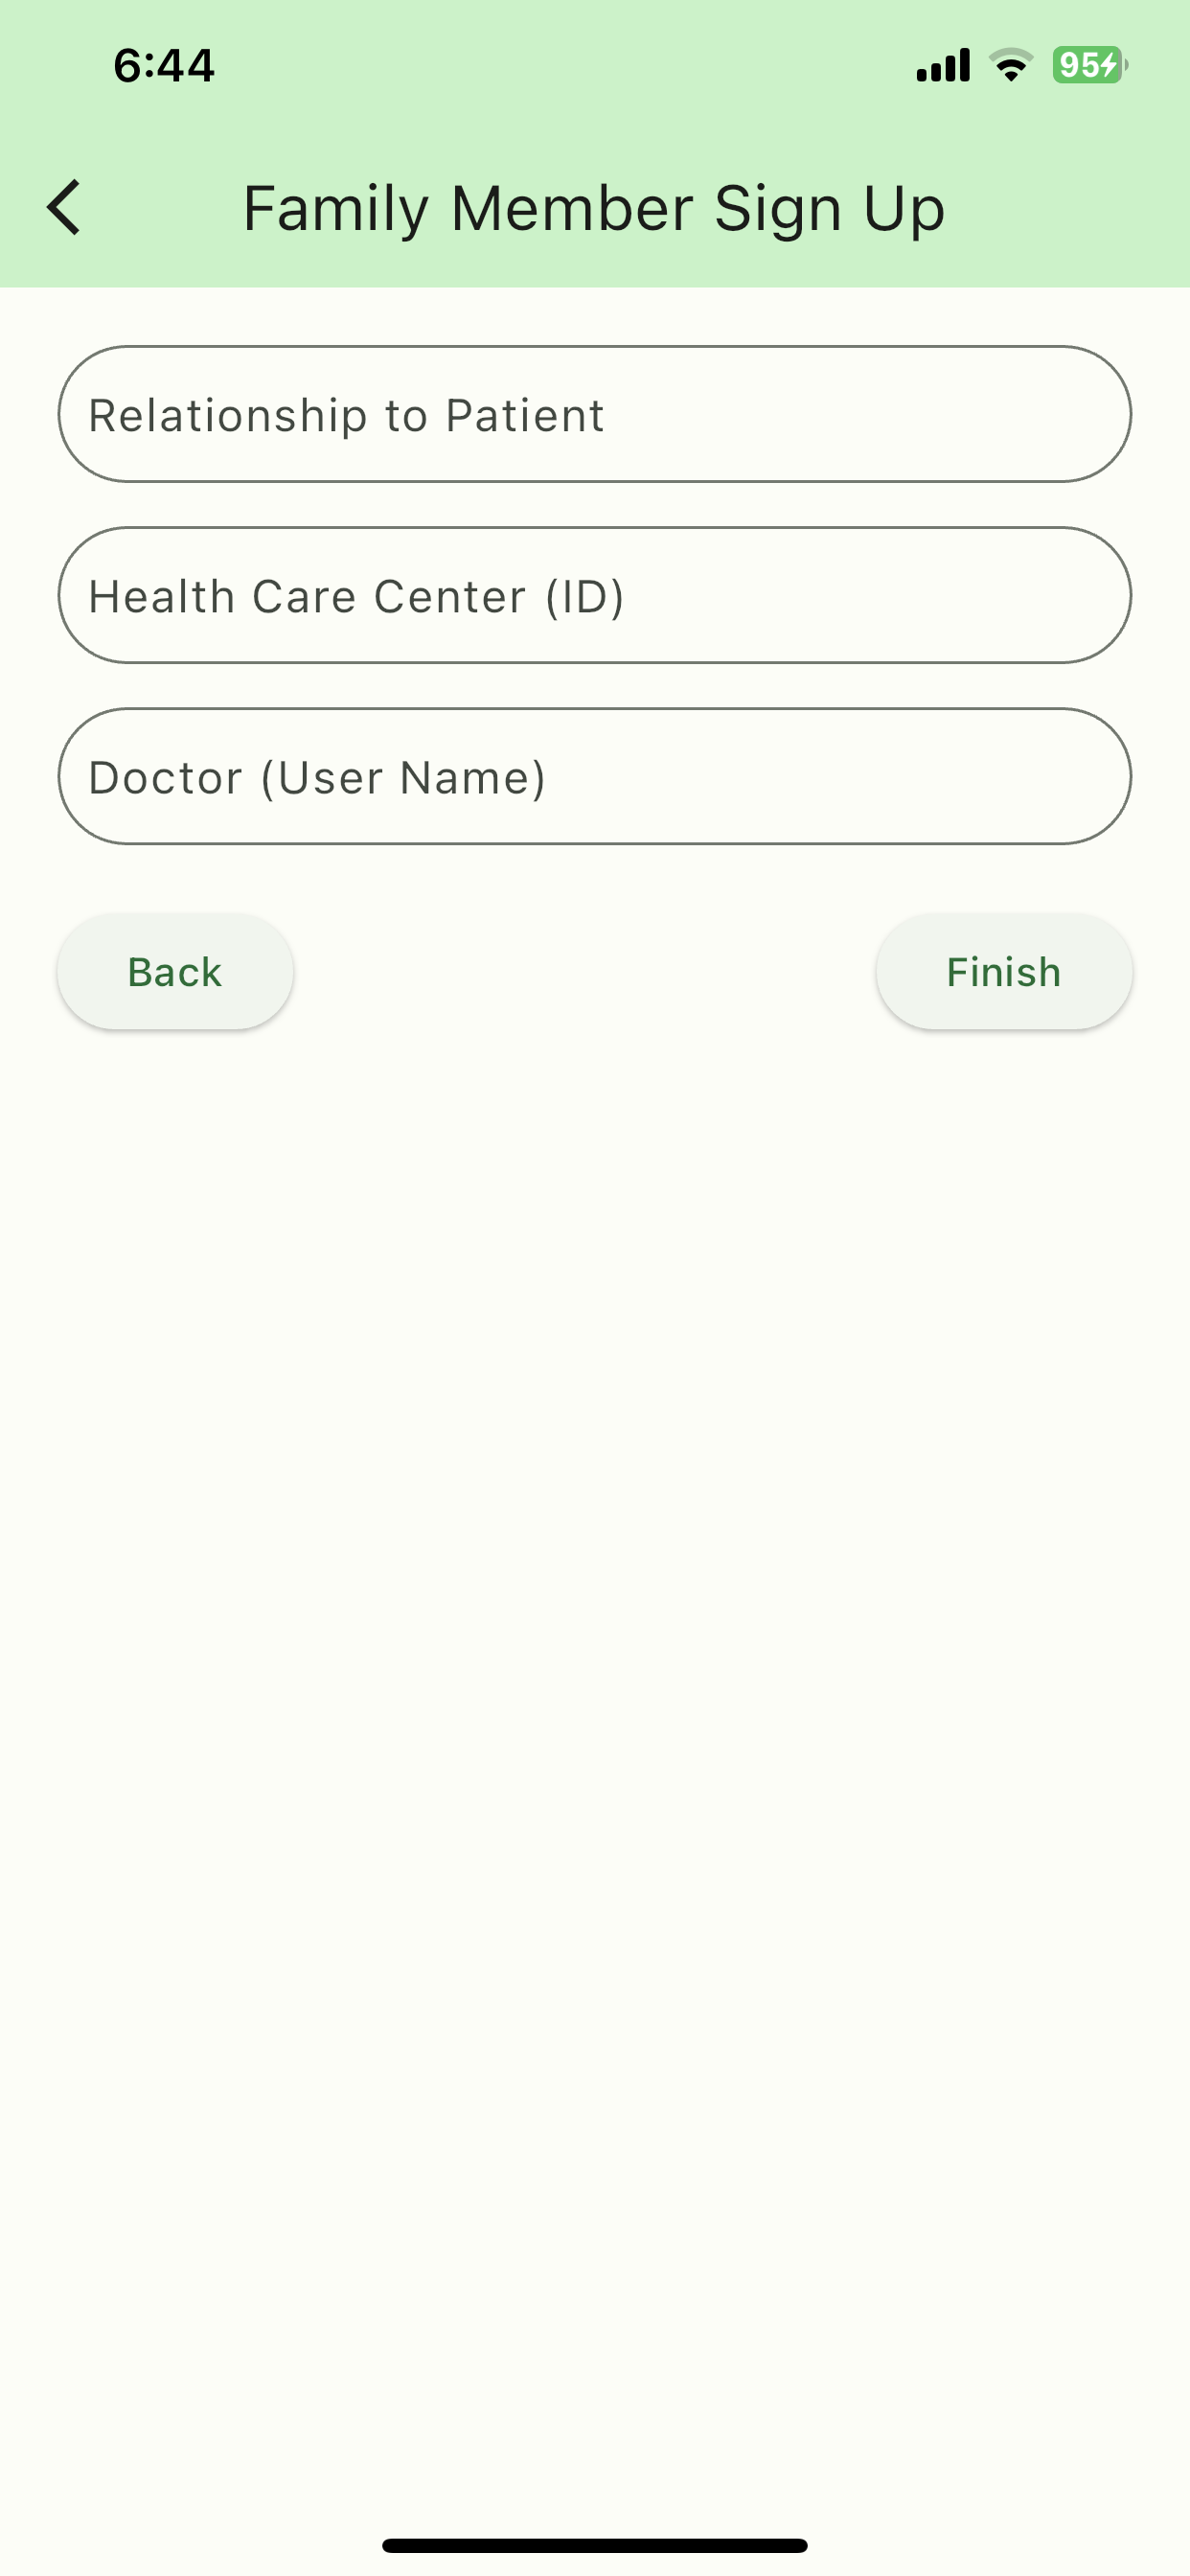
\includegraphics[width=.5\linewidth]{SignUpFamilyMember.png}
		\caption{SignUp Family Member1}\label{SignUp Family Member}
	\end{minipage}
\end{figure}
	\begin{figure}[!h]
	\centering
	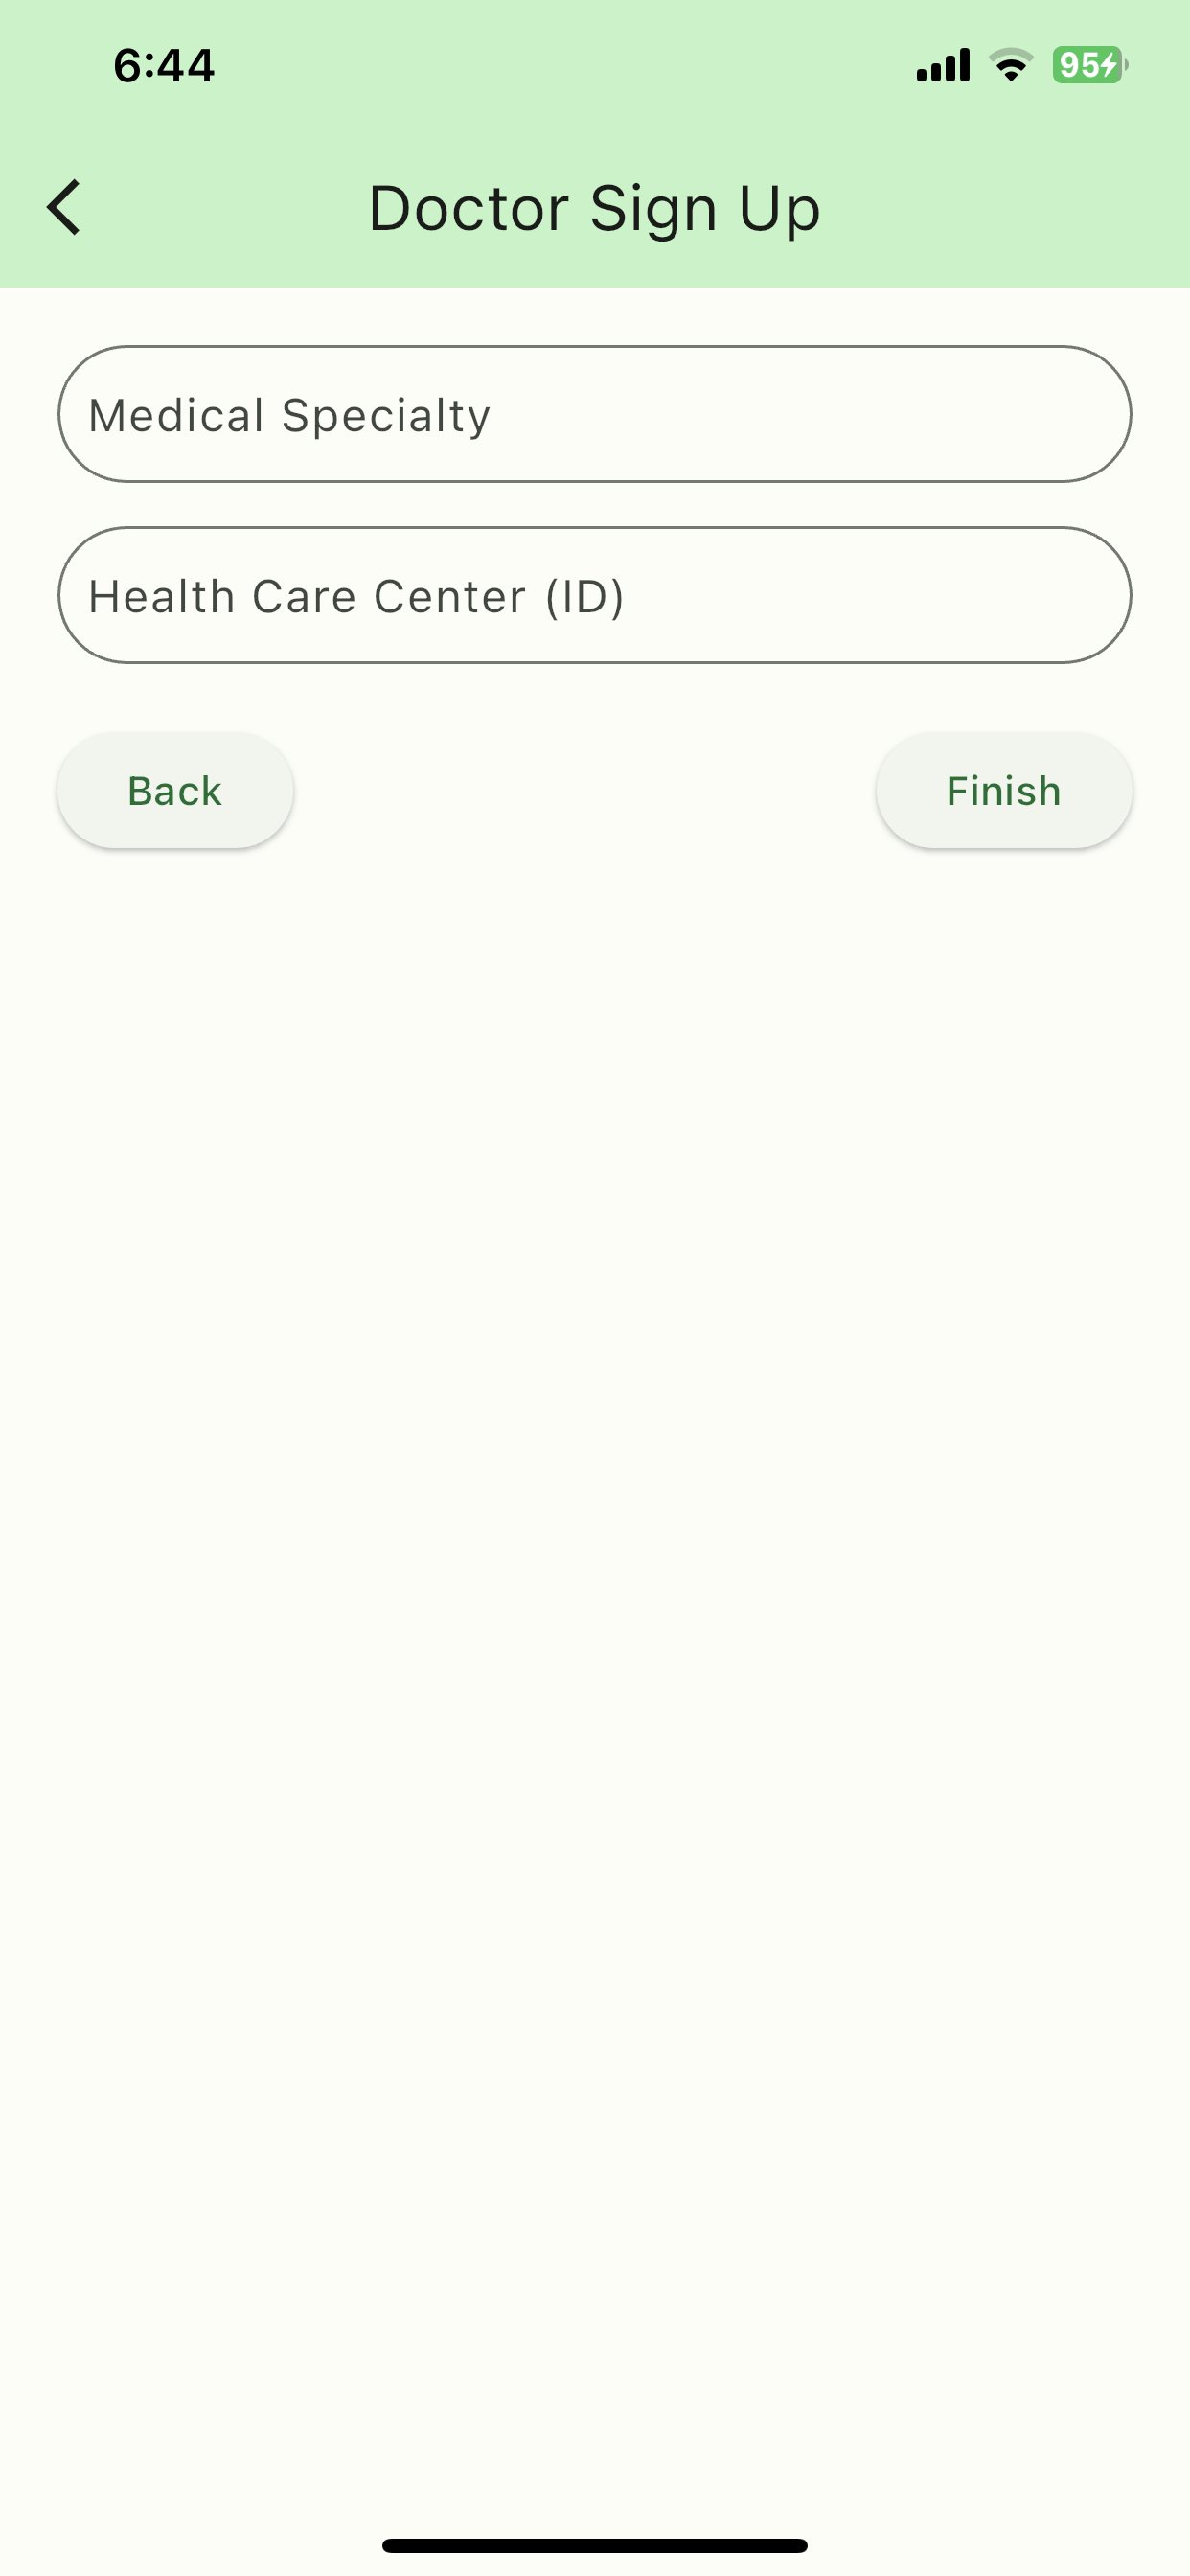
\includegraphics[width=0.25\textwidth]{SignUpDoctor.png}
	\caption{SignUp Doctor}
	\label{SignUp Doctor}
\end{figure}
\newpage
\textbf{\underline{Patient screens:}}
\begin{figure}[!htb]
	\begin{minipage}{0.48\textwidth}
		\centering
		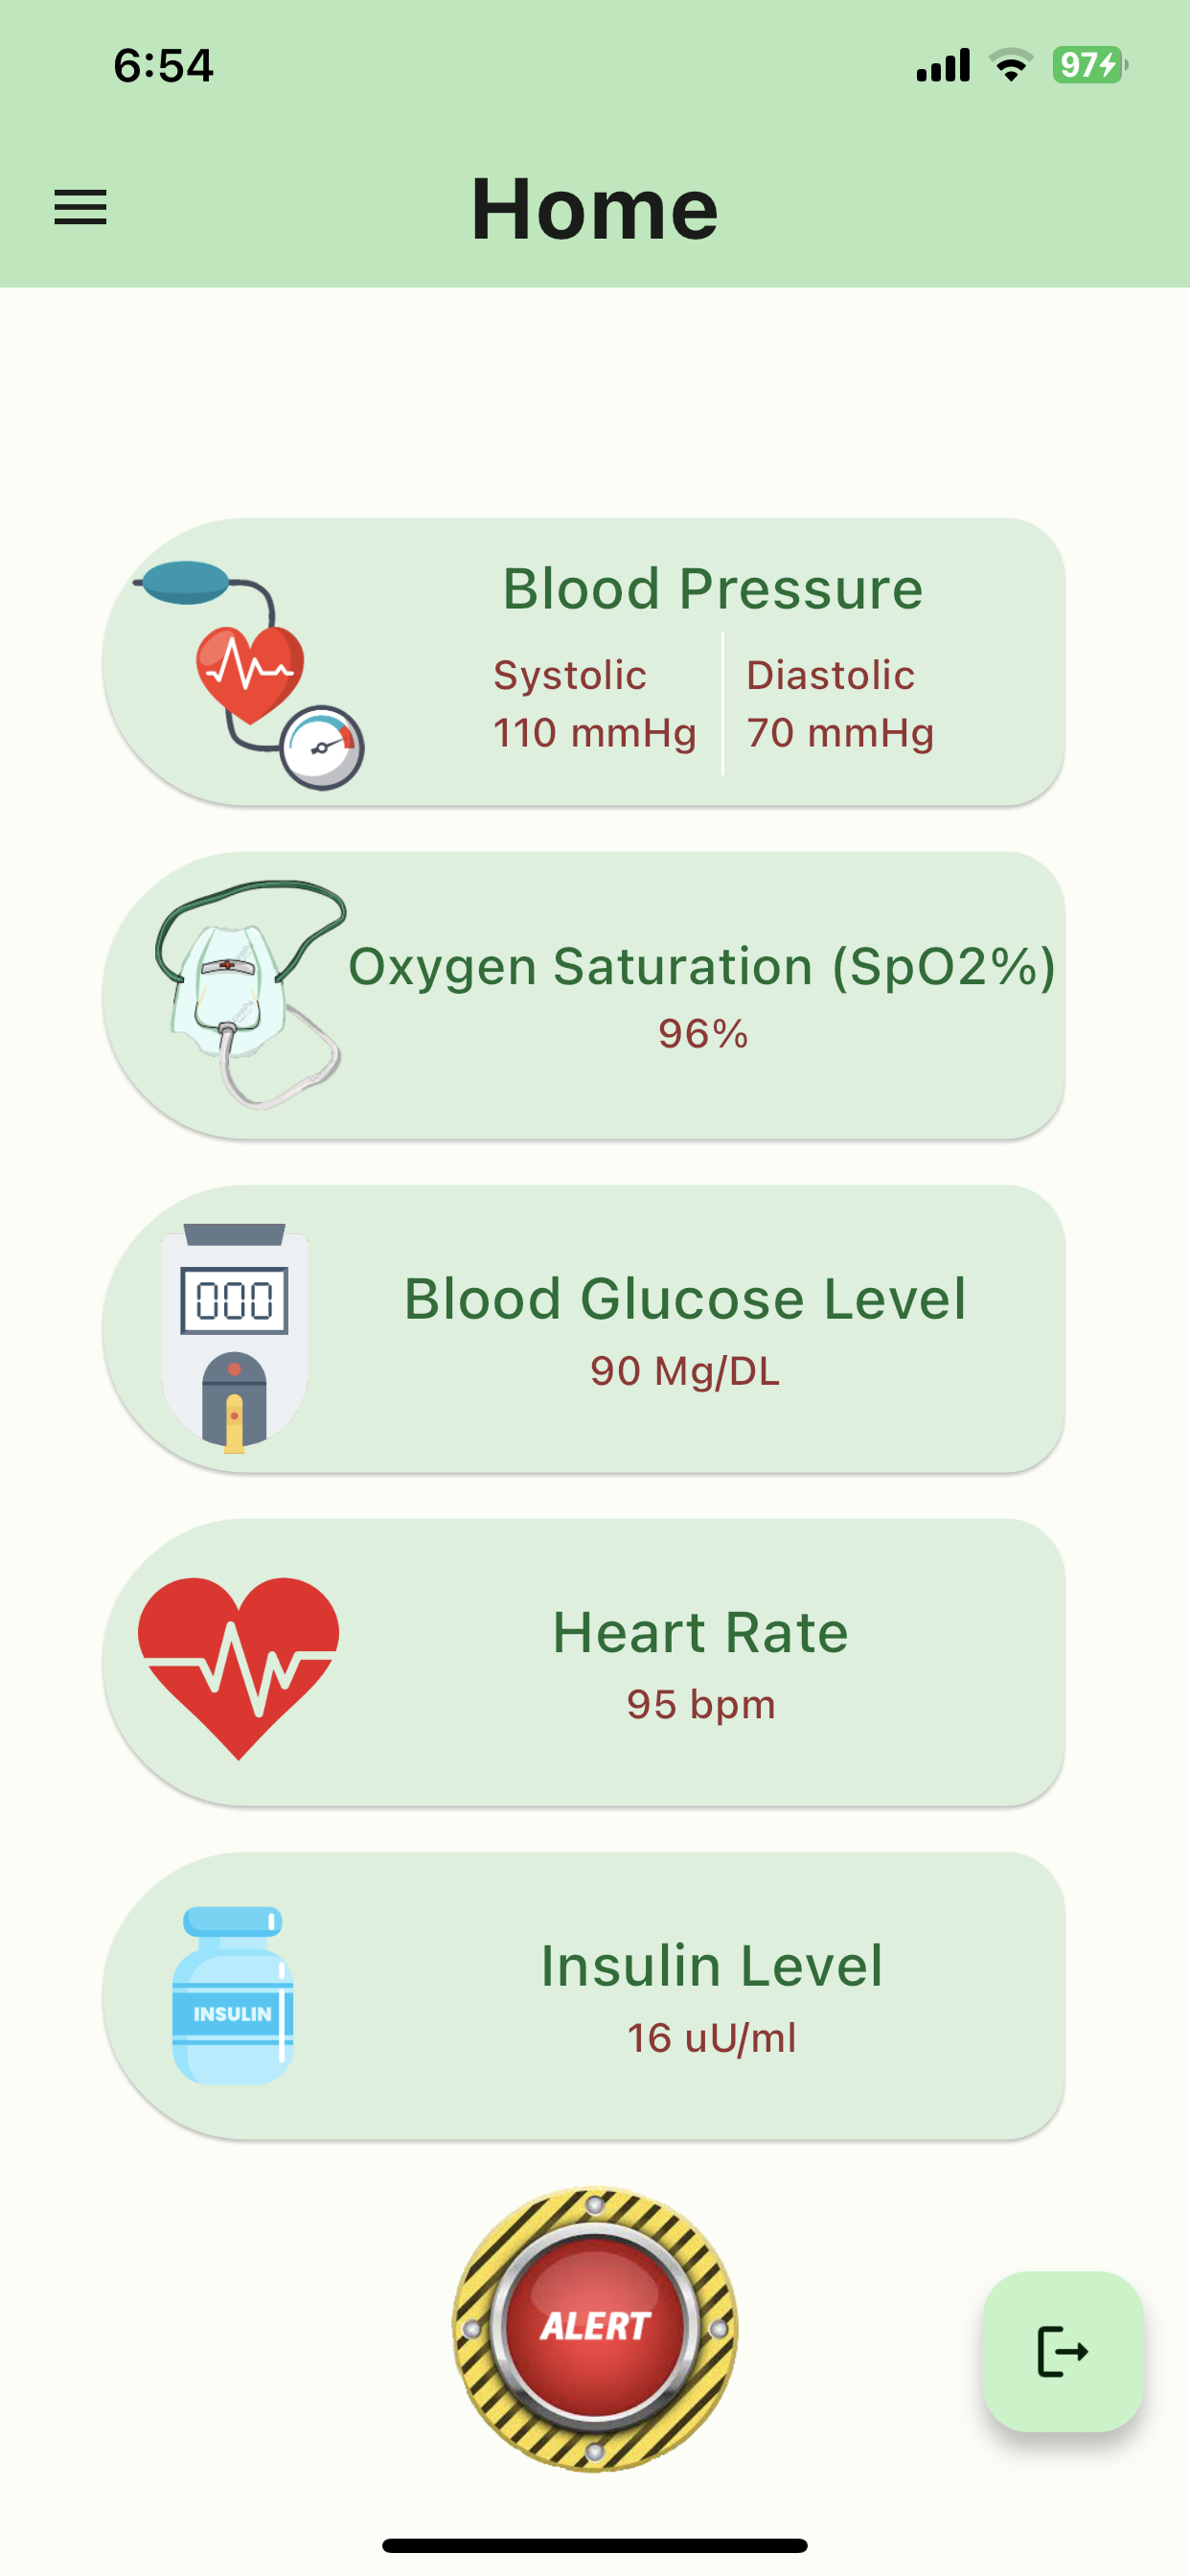
\includegraphics[width=.5\linewidth]{PatientHome.png}
		\caption{Patient Home}\label{Patient Home}
	\end{minipage}\hfill
	\begin{minipage}{0.48\textwidth}
		\centering
		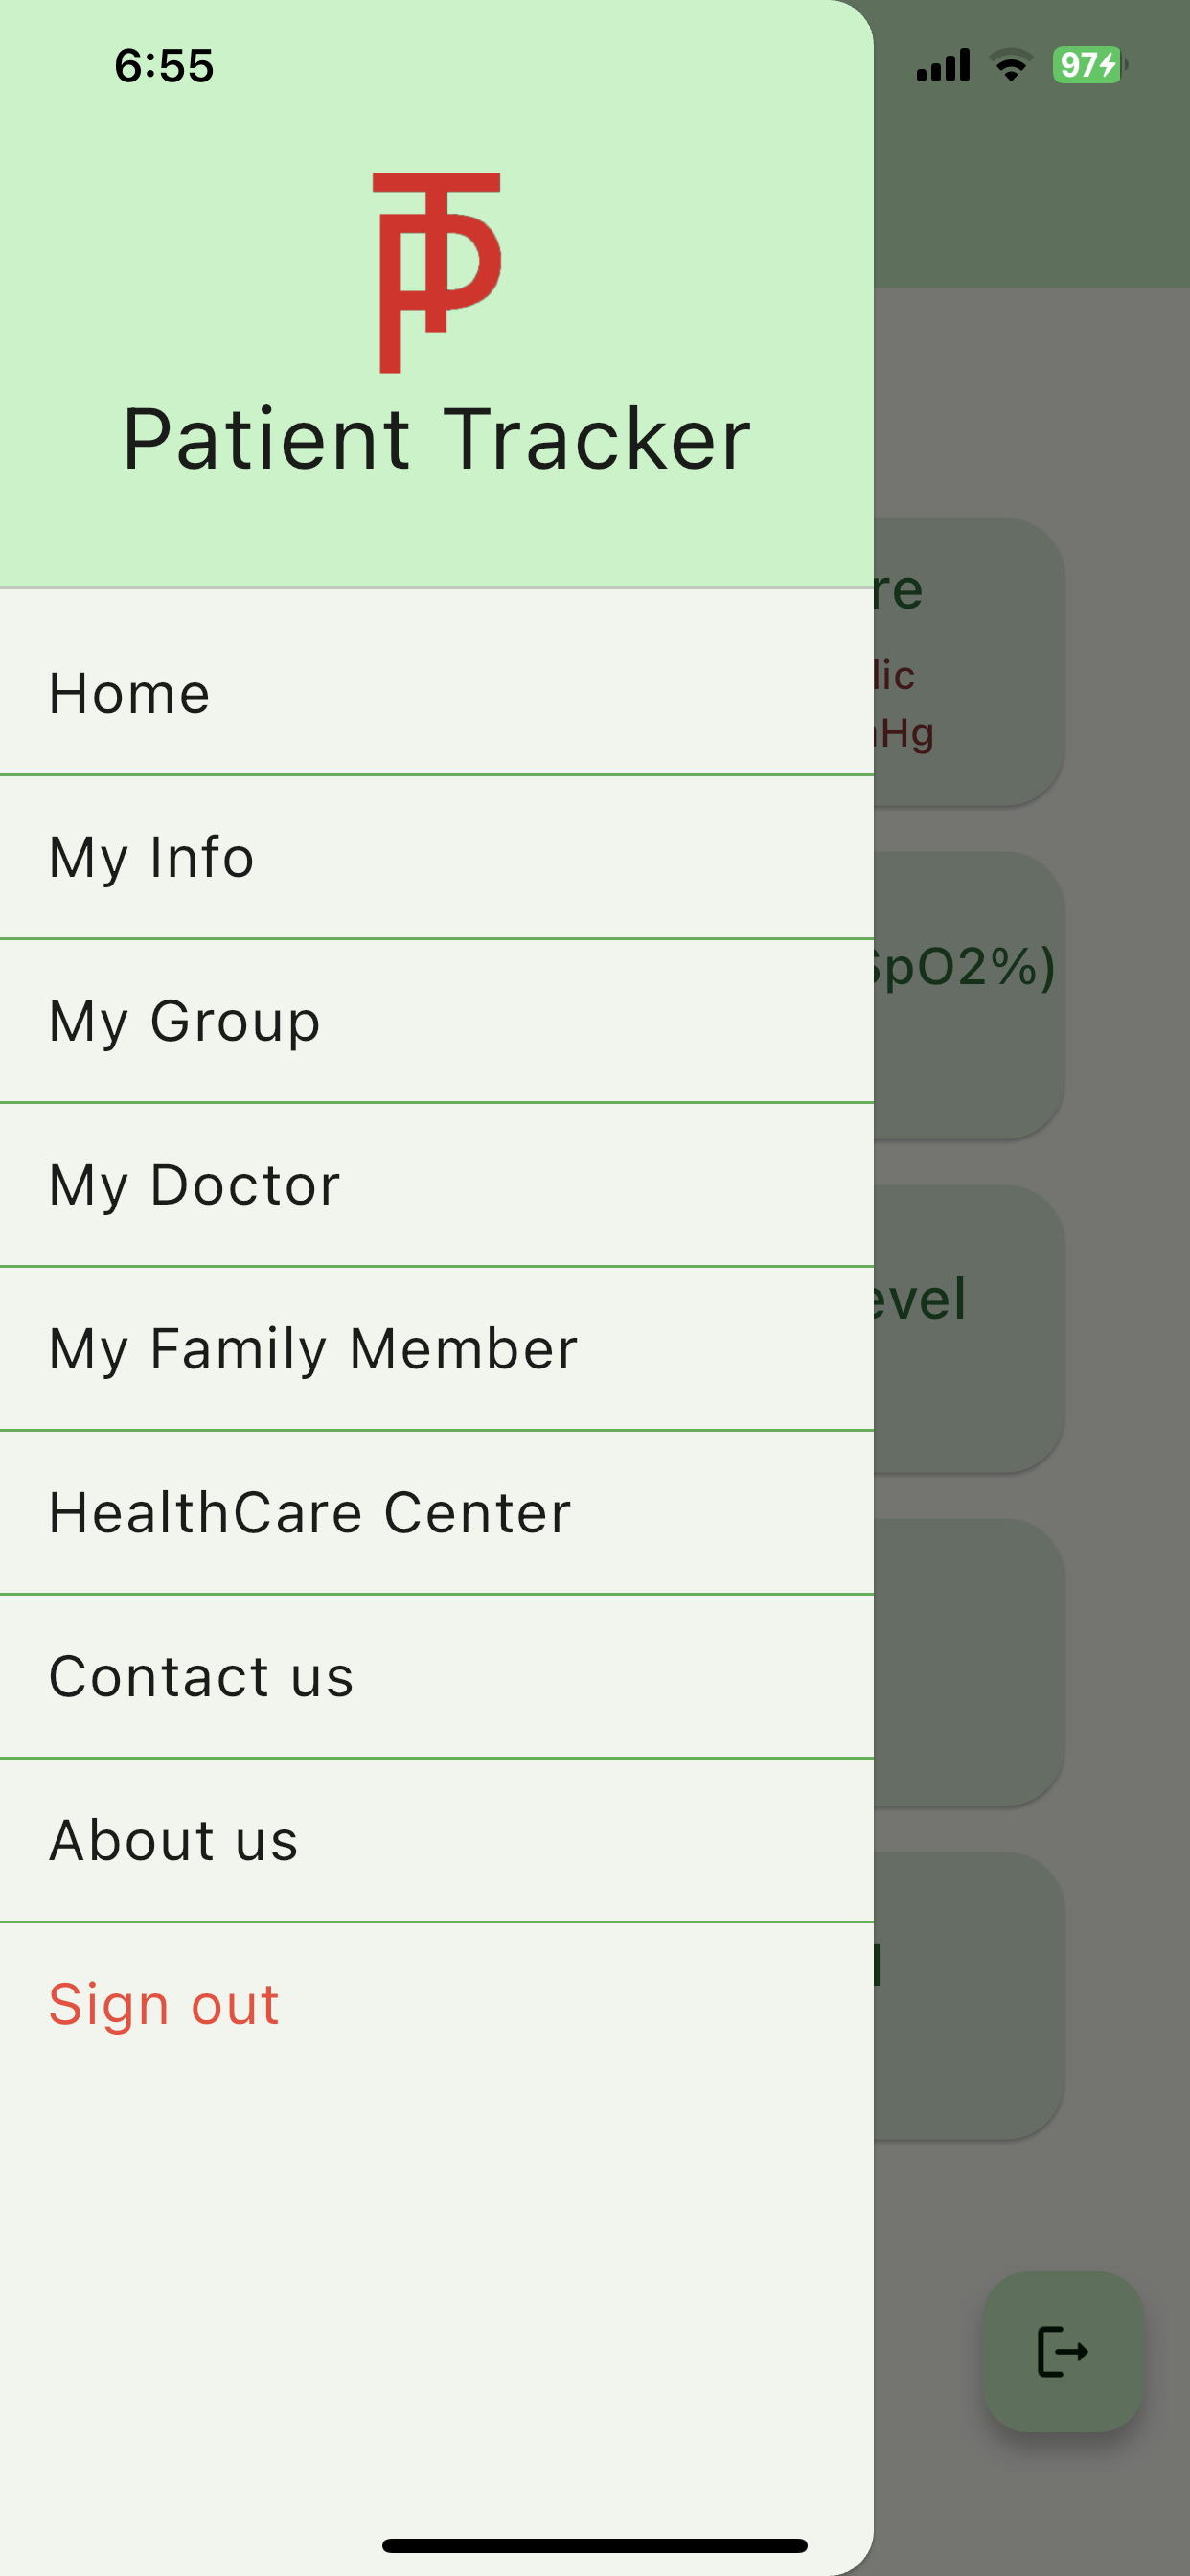
\includegraphics[width=.5\linewidth]{PatientDrawer.png}
		\caption{Patient Drawer}\label{Patient Drawer}
	\end{minipage}
\end{figure}
			\subsection{Summary}
			
			\quad System development for a patient tracker system involves the design, development, and
			implementation of software solutions to effectively monitor and manage patient 
			information in healthcare settings. It aims to improve patient care by providing healthcare
			professionals with a reliable platform for tracking and recording patient data, facilitating
			communication, and streamlining administrative tasks. 
			
			Successful system development
			leads to enhanced patient outcomes, improved communication among healthcare
			providers, and increased efficiency in delivering healthcare services.
			\newpage
			\section*{\begin{center}
					Chapter Six
			\end{center}}
			\section{TESTING}
			\subsection{Introduction}
			
			\quad System testing plays a crucial role in the development of a patient tracker system. It is a
			comprehensive and structured process that evaluates the functionality, performance, and
			reliability of the system to ensure its effectiveness in managing patient information. The
			main objective of system testing is to identify and resolve any defects, errors, or
			inconsistencies in the system before it is deployed for actual use. Through rigorous
			testing, the patient tracker system can be validated for accuracy, security, and usability,
			ultimately ensuring that it meets the needs and expectations of healthcare professionals
			and provides reliable and efficient patient tracking capabilities.
			
			\subsection{System Testing}
			\quad System testing is an essential part of software development that involves testing the entire system or software application as a whole to ensure that it meets the required specifications and functions properly. Different types of system testing, such as functional testing, performance testing, security testing, and usability testing, are performed to verify the system's quality, reliability, and integrity.
			
			here are the different types of system testing that can be performed for a patient tracker app:
			\begin{itemize}
				
		
			\item 	Functional testing: This type of testing verifies that the app is functioning correctly and all the features are working as expected. It includes testing of features like user authentication, data collection and storage, location tracking, data visualization, and alerting.
			
			\item 	Usability testing: This type of testing is done to evaluate the app's ease of use, user interface, and user experience. It involves testing the app's navigation, layout, responsiveness, and overall design.
			
			\item 	Performance testing: This type of testing is done to measure the app's performance under different conditions. It includes testing the app's speed, stability, and scalability, and how it handles a large number of users.
			
			\item 	Security testing: This type of testing is done to identify and address potential security vulnerabilities in the app. It includes testing the app's encryption, data transmission, user authentication, and access control.
			
			\item 	Compatibility testing: This type of testing is done to ensure that the app is compatible with different devices, operating systems, and network environments. It involves testing the app on various platforms and devices to ensure it works as expected.
			
			\item 	Regression testing: This type of testing is done to ensure that the app's new features or updates do not break the existing functionality. It involves testing the app after each change or update to ensure that it is still functioning as expected
			
			\quad Performing all of these types of system testing can help ensure the quality, functionality, and security of the patient tracker app.
			
			
			\quad Also, it is important to have a well-defined testing plan and test cases to ensure that all aspects of the app are thoroughly tested
			
			\quad Automated Testing: Automated testing involves using software tools to test the app automatically. This method can be used to test app functionality, performance, and scalability. Automated testing is a good option for large projects or projects that require frequent testing, as it is more efficient than manual testing. However, it can be expensive and may require specialized knowledge and resources.
			
			\quad Automated testing is useful for the patient tracker app because it allows for faster and more consistent testing of the app's functionality, ensuring that the app meets the necessary quality standards before deployment. Since patient tracker apps often deal with sensitive personal health information and have real-world implications for patient health and safety, it is important to thoroughly test the app's functionality to ensure that it works as intended and that patient data is kept secure.
			
			\quad Automated testing can be used to simulate real-world scenarios and test various aspects of the app's functionality, such as user authentication, data encryption, GPS tracking, and notifications. By automating these tests, developers can easily and consistently test the app's functionality, which can help catch bugs and other issues before they become bigger problems.
			
			\quad Additionally, automated testing can help reduce the risk of human error in testing, as automated tests are typically more reliable and consistent than manual testing. This can help improve the app's overall quality and reduce the risk of errors or issues that could potentially harm patient health or compromise sensitive patient data.
			
			
			\quad Manual testing is best for patient tracker apps in certain scenarios, such as when testing the user interface and user experience. This is because human testers can more easily identify visual and usability issues that automated testing tools may not be able to detect. 
			
			\quad Manual testing can also be useful for testing the app's functionality in specific use cases and scenarios that automated testing may not easily cover. In addition, manual testing can provide valuable feedback on the overall quality and usability of the app from the perspective of a real user. However, manual testing can also be time-consuming and resource-intensive, which is why it is often used in combination with automated testing to achieve a more comprehensive testing approach.
			
			
			
			\quad By combining both manual and automated testing, we can achieve a more comprehensive testing approach that covers a wider range of scenarios and increases the chances of detecting and fixing any issues in the patient tracker app. Manual testing can also help identify usability issues and provide feedback on the app's overall user experience, while automated testing can help catch bugs quickly and efficiently.
			
			
			\end{itemize}
			\subsection{System Integration}
			\quad System integrity for a patient tracker app refers to the ability of the app to maintain the confidentiality, availability, and accuracy of patient data. This includes ensuring that the app is secure and that only authorized users have access to patient data. It also involves implementing measures to prevent data loss, data corruption, and unauthorized modification of data. In addition, the app must be designed to function reliably and with high availability so that patient data can be accessed and used as needed. Overall, system integrity is critical for patient tracker apps to ensure that patient data is protected and that the app functions effectively to support patient care.\\
			
			\quad Automated testing can help ensure the integrity of the data in a patient tracker app by detecting any potential bugs or errors in the code that could compromise the security or accuracy of the data. Automated tests can be run on a regular basis to check that the app is functioning properly and that the data being collected and stored is accurate and secure. This can help catch any issues early on before they become major problems, allowing developers to quickly address any issues and ensure that the app is operating as intended. Additionally, automated testing can help reduce the risk of human error, which can be a major factor in data integrity issues.
			\subsection{System Testing Result}
			
			\quad The system testing result for a patient tracker app that has undergone both automated and manual testing, with a focus on maintaining data integrity, would likely be a more robust and reliable application. The combination of automated and manual testing can provide a more comprehensive approach to identifying and addressing potential issues or bugs, as well as ensuring that the app meets the requirements and needs of its users. Additionally, maintaining data integrity is crucial for a patient tracker app, as it involves sensitive and confidential information. By using both automated and manual testing, the app's functionality and data security can be thoroughly evaluated and improved. Ultimately, this can result in an app that is more trustworthy and effective in tracking patient health and wellness.
			\subsection{Summary}
			
			\quad Automated testing can quickly and efficiently identify issues in patient tracker apps, while manual testing allows for a more thorough examination of user experience. The combination of both testing methods can provide comprehensive results and help ensure the integrity of the app's data. Security measures, such as encryption and secure data storage, are also important for maintaining data integrity.
			
			\section*{\begin{center}
					Chapter Seven
			\end{center}}
			\section{CONCLUSION AND FUTURE WORKS}
			\subsection{Conclusion}
			
			\quad The patient tracker app is a powerful and comprehensive solution for managing and
			tracking patient information in the healthcare sector. It offers a range of features and
			functionalities that enhance communication, streamline processes, and improve overall
			patient care.
			With its user-friendly interface and intuitive design, the app provides healthcare
			professionals with quick and easy access to vital patient data. It allows for efficient
			tracking of patient demographics, medical history, vital signs, and current health status.
			
			This information empowers healthcare providers to make informed decisions, deliver
			personalized care, and monitor patient progress effectively.
			Through the integration of automated and manual testing, the app ensures the integrity
			and accuracy of patient data. It undergoes rigorous testing to identify and address
			potential issues or bugs, ensuring the app operates as intended and meets the needs of
			healthcare professionals and patients.
			The patient tracker app also plays a vital role in patient engagement and selfmanagement. It allows patients to input their medical information, track changes in their
			health, and receive relevant notifications and reminders. This promotes proactive
			healthcare management, empowers patients to take charge of their well-being, and
			fosters a collaborative patient-provider relationship.
			Furthermore, the app enhances communication and collaboration among healthcare team
			members. 
			
			It enables seamless sharing of patient information, facilitates real-time updates,
			and supports remote monitoring. This ensures that healthcare providers and caregivers
			stay connected, enabling timely interventions and coordinated care.
			In conclusion, the patient tracker app revolutionizes healthcare management by providing
			a comprehensive platform for efficient patient tracking, secure data management, and
			improved communication. It empowers healthcare professionals, engages patients in their
			own care, and ultimately contributes to better health outcomes. With its innovative
			features and focus on patient-centered care, the patient tracker app is poised to
			transform the healthcare landscape.
			\subsection{Future Works}
			
			While the patient tracker app has made significant strides in improving patient care and
			healthcare management, there are several areas of future work that will enhance its
			functionality and expand its reach.
			\begin{itemize}
			\item  Security and Validation: As patient data security and privacy continue to be
			paramount concerns, ongoing efforts will focus on strengthening the app's security
			measures. This includes implementing robust encryption protocols, ensuring secure
			data storage and transmission, and conducting regular security audits. Additionally,
			continuous validation of the app's data inputs and outputs will be essential to
			maintain data integrity and prevent any vulnerabilities or unauthorized access.
			\item Full Testing and Quality Assurance: Although the app has undergone extensive
			testing, continuous testing, and quality assurance will remain a crucial aspect of its
			development. This includes performing comprehensive end-to-end testing, stress
			testing, and performance optimization. By identifying and resolving any potential
			issues, the app can deliver a seamless and reliable experience to healthcare
			providers and patients.
			\item  Android Compatibility: While the initial focus may have been on the iOS system,
			future work will involve developing an Android version of the patient tracker app. 
			This expansion will allow a broader range of users to access and benefit from its
			features, thereby increasing its overall impact and reach in the healthcare sector.
			\item  Excluded Functions: Throughout the development process, certain functions may
			have been excluded from the initial release to prioritize core features and ensure a
			seamless user experience. Future work will involve revisiting these excluded
			functions and incorporating them into the app's roadmap. This could include
			additional features such as medication reminders, instructions on first aid,
			appointment scheduling, integration with wearable devices, and telemedicine
			capabilities, among others.
			\end{itemize}
			
			By addressing these areas of future work, the patient tracker app will continue to evolve
			and adapt to the changing needs of the healthcare industry. With enhanced security,
			expanded platform compatibility, and the inclusion of additional functions, the app will
			continue to play a pivotal role in revolutionizing patient care, improving outcomes, and
			empowering both healthcare providers and patients.
	\bibliographystyle{IEEEtran}
	\bibliography{references}
\end{document}